\documentclass[11pt, oneside]{article}   	
\usepackage[margin=1in]{geometry}                		
\geometry{a4paper}                   		
%\usepackage[spanish, es-noindentfirst]{babel}
%\selectlanguage{spanish}
%\usepackage[utf8]{inputenc}               		
    		
\usepackage{graphicx}	
\usepackage{caption}
\usepackage{subcaption}		
\usepackage{float}	
										
\usepackage{amssymb}
\usepackage{amsmath}
\usepackage{authblk}
\usepackage{bm}
%\usepackage[lite]{mtpro2}

\usepackage{booktabs}

\usepackage{geometry}
\geometry{lmargin=0.75in,rmargin=0.75in,tmargin=1in,bmargin=0.65in}
\usepackage{setspace}
\usepackage{multirow}

\pagenumbering{gobble}
\usepackage{verbatim}
\immediate\write18{texcount -tex -sum  \jobname.tex > \jobname.wordcount.tex}

% Keywords command
\providecommand{\keywords}[1]
{
  \small	
  \textbf{\textit{Keywords:}} #1
}


\newcommand{\bx}{\mathbf{x}}
\newcommand{\bu}{\mathbf{u}}
\newcommand{\bz}{\mathbf{z}}
\newcommand{\bA}{\mathbf{A}}
\newcommand{\bX}{\mathbf{X}}
\newcommand{\bY}{\mathbf{Y}}
\newcommand{\bV}{\mathbf{V}}
\newcommand{\bv}{\mathbf{v}}
\newcommand{\bbeta}{\bm{\beta}}
\newcommand{\myeta}{\bm{\eta}}
\newcommand{\indep}{\rotatebox[origin=c]{90}{$\models$}}

\usepackage{mathpartir}
\usepackage{etoolbox}

\newcommand{\zerodisplayskips}{%
  \setlength{\abovedisplayskip}{2pt}
  \setlength{\belowdisplayskip}{2pt}
  \setlength{\abovedisplayshortskip}{2pt}
  \setlength{\belowdisplayshortskip}{2pt}}
\singlespacing

\usepackage{pifont}
\newcommand{\cmark}{\ding{51}}%
\newcommand{\xmark}{\ding{55}}%
\usepackage{booktabs}
\usepackage{subcaption}

\title{Estimation of average treatment effect for ACIC data challenge}
\author[]{Wanwan Xu}
\affil[]{Univeristy of Connecticut, Department of Statistics}
\renewcommand\Authands{, }
\date{}							


\begin{document}
\maketitle

\begin{abstract}
This is a data-driven project based on ACIC 2019 data challenge, the main objective is to estimate the population average treatment effect (ATE). The performance of regression estimator, inverse propensity weighted estimator, augmented inverse propensity weighted estimator and calibration estimator is compared on test datasets as well as some theoretical properties. The final result for all 3,000 sets of training data is also presented. 
\end{abstract}
\keywords{average treatment effect, counterfactual, causal inference}

\section{Introduction}
Treatment effect has always been of interest, as it quantitatively  show the causal effect of a binary variable on an outcome variable. This variable, although with name `treatment'', is now used much more generally than a medical procedure or experimental drug. In economics, the causal effect of a subsidized training program \cite{Ashenfelter1978} is widely analyzed, so are the effects of active labor market programs such as job search assistance or classroom teaching program \cite{LaLonde1986}. Since treatment effect is defined as the difference between two treatment groups, while in reality, one unit or one observation is only related to one of the treatment assignment, it's impossible to measure causal effects at the individual level, therefore we focus on the expectation, i.e. average treatment effect(ATE):
$$\mbox{ATE}=E[Y_{1i}-Y_{0i}]=E[E(\bY | \bA = 1, \bV) - E(\bY | \bA = 0, \bV)]$$
where $\bY$ is the response variable, $\bA$ is treatment variable and $\bV$ is the set of covariates. 

A typical concern for inferring causality in an observational study is confounding, treatment exposure may be associated with covariates that are also associated with potential response. For example, experiment individual characteristics such as demographic factors can be related to both the treatment selection and the outcome of interest. In order to perform unbiased comparison despite the confounding factors, the inferences with causal interpretation need to be adjusted. There are three broad classes of strategies: (1) Outcome regression \cite{Oaxaca1973}. The model of outcome $\bY$ given covariates $\bV$ need to be specified, it follows similar procedure of calculating counterfactuals. (2) Propensity score estimation \cite{Rosenbaum1983}. This method requires the construction of weights for individual observations via using estimated propensity scores \cite{Robins2000}, then use the average of within stratum effects as ATE \cite{Rosenbaum1984}. (3) Non-parametric estimation \cite{Chan2016}. The authors applied the class of survey calibration estimators on the estimation of average treatment effects, they also showed that a globally efficient estimator can be adapted from it. 

This report focuses on applying several estimation methods described above to ACIC data challenge low dimension track datasets. The report is organized as follows. In Section \ref{sec:data}, we introduce the data structure and explanation. The methods applied is briefly introduced in Section \ref{sec:method}, the comparison based on test dataset is presented in Section \ref{sec:result} as well as the results for training dataset. Some final remarks and future directions are given in Section \ref{sec:disc}.
\section{Dataset}\label{sec:data}
\subsection{Introduction}
Two tracks of data (low dimension and high dimension) are included in the ACIC data challenge, each track have 3200 csv files drawn from 32 unique data generating processes (DPG). In this report, we focus only on low dimensional track. Within each csv file, there are:
\begin{itemize}
\setlength\itemsep{-0.5em}
\item response variable $\bY=\{Y_1,Y_2,\ldots,Y_n\}$, half are continuous while the other half is discrete;
\item binary treatment indicator $\bA=\{A_1,A_2,\ldots,A_n\}$;
\item pre-treatment covariates $\bV=\{V_1,\ldots,V_p\}$, which includes the mixture of continuous, binary, and categorical variables.
\end{itemize}
Aside from the mixture of data type, number of covariates and number of observations may also be different for each worksheet as shown in Figure \ref{fig:pie}.
\begin{figure}[]
\begin{subfigure}{.5\textwidth}
  \centering
  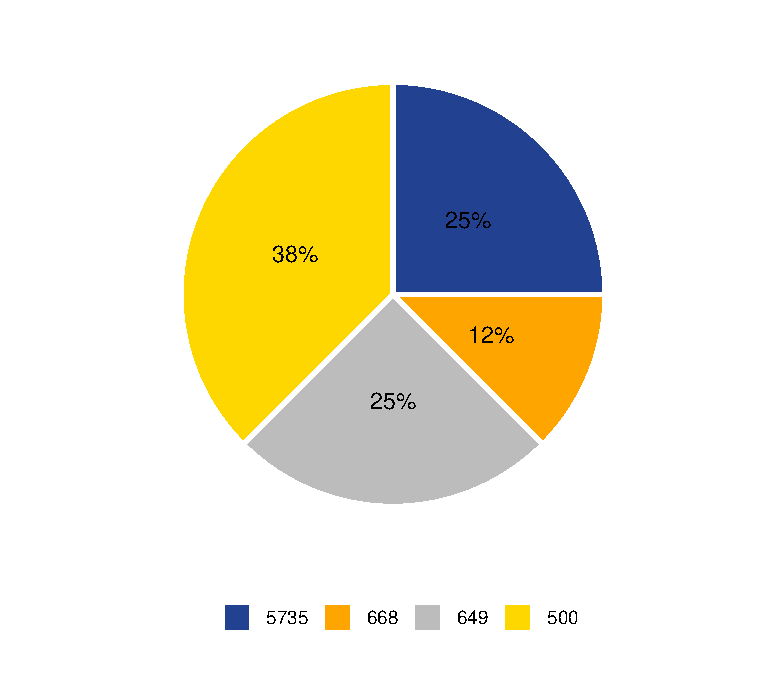
\includegraphics[width=1\linewidth]{../plot/obs_freq}
  \caption{number of observations}
\end{subfigure}%
\begin{subfigure}{.5\textwidth}
  \centering
  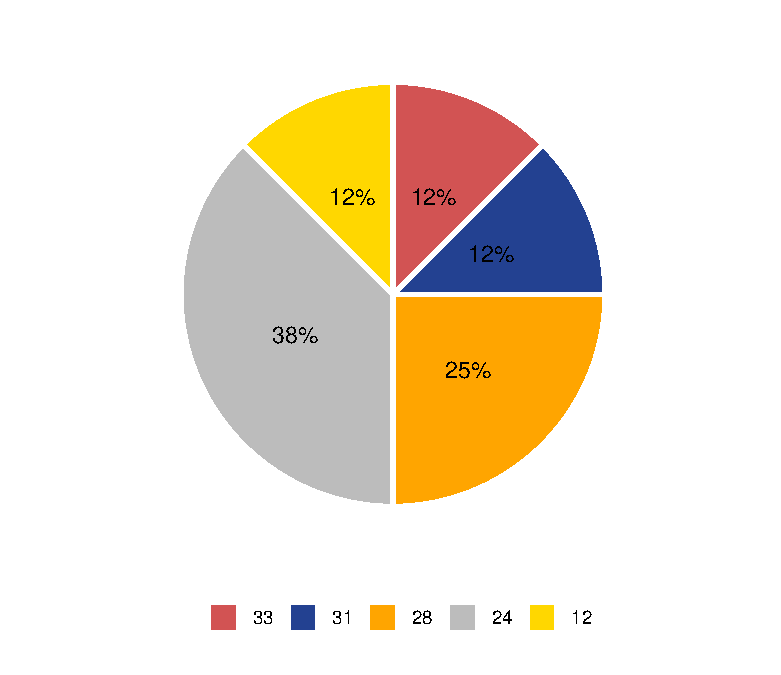
\includegraphics[width=1\linewidth]{../plot/var_freq}
  \caption{number of covaraibles}
\end{subfigure}
\caption{Frequency plot low track dataset}
\label{fig:pie}
\end{figure}
The description site of data challenge also provided some more information. For instance, there are no mediators among covariates, that is we only need to consider direct effect from covariates. Also, all the covaraites also include all the cofounders, we don't need to consider hidden variables. However, selection variables may still exists, given some of the covaraites may be related to the treatment factor $\bA$.
\subsection{Objectives}
The measure of estimation is the population average treatment effect (ATE) and 95\% confidence interval for each dataset. For individual $i \in \{1,2,\ldots,n\}$, denote $Y_{0i}$ as the outcome variable for individual $i$ if he/she is not treated, $y_{1i}$ as the value of the outcome variable for individual $i$ if he/she is treated. The treatment effect for individual $i$ is given by $Y_{1i}-Y_{0i}=\beta_i$. In the general case, there is no reason to expect this effect to be constant across individuals. The average treatment effects is given by $\mbox{ATE}=E[Y_{1i}-Y_{0i}]$, where the expectation is with respect to the distribution of covariates. 

However, in observational data, we can only observe one of the two for each individual, thus estimation techniques are needed. Under this circumstances, one of the $y_{0i},y_{1i}$ will be replaced by counterfactual output. Since the causal assumptions of consistency and strong ignorability are guaranteed, the target statistical estimate can be rewritten as: $\mbox{ATE}=E[E(\bY | \bA = 1, \bV) - E(\bY | \bA = 0, \bV)]$.
\section{Method}\label{sec:method}
\subsection{Basic models}
As presented before, I compared a few different methods on the ATE estimation$\mbox{ATE}=E[E(\bY | \bA = 1, \bV) - E(\bY | \bA = 0, \bV)]$, including:

\noindent
\textit{\textbf{Outcome model (REG)}}:

Lots of traditional causal estimation relies on the formulation of a regression model for the outcome variable $\bY$. In other words, the focus is on the estimation of $E[\bY|\bA,\bV]$. Given ATE is defined with respect to the distribution of covariates, the empirical distribution will be an easy estimate of $F_{\bV}$. Thus the regression estimate can be written as:
$
\widehat{\mbox{ATE}}_{REG}=\frac{1}{n}\sum_{i=1}^n \{\hat{E}(\bY | \bA = 1, V_i) - \hat{E}(\bY | \bA = 0, V_i)\}
$

\noindent
\textit{\textbf{Propensity score model (IPW)}}:

Due to the limitation of regression estimator, another widely applied method for estimating ATE relies on a model for treatment
assignment instead a regression model for the outcome was proposed. Suppose the true probability of assigning treatment were known, this could be used to define propensity scores, and further be used for matching or weighting covariates. A well-known weighting estimator is the IPW estimator:
$\widehat{\mbox{ATE}}_{IPW} =\left\{\sum_{i=1}^n \frac{A_i}{\hat{\pi}(\bV_i)}\right\}^{-1}\sum_{i=1}^n \frac{A_iY_i}{\hat{\pi}(\bV_i)} -\left\{\sum_{i=1}^n \frac{1-A_i}{1-\hat{\pi}(\bV_i)}\right\}^{-1}\sum_{i=1}^n\frac{(1-A_i)Y_i}{1-\hat{\pi}(\bV_i)}
$

\noindent
\textit{\textbf{AIPW model}}:

Based on the previous work of IPW estimation, one improvement including fully utilizing the information in the conditioning set $\bV$ is AIPW \cite{Glynn2010}. Aside from the information about treatment assigning probability, $\bV$ also carry the predictive information about the response variable $\bY$:
\begin{align*}
\widehat{\mbox{ATE}}_{AIPW} = \frac{1}{n}\sum_{i=1}^n & \bigg\{\left[ \frac{A_iY_i}{\hat{\pi}(\bV_i)}-\frac{(1-A_i)Y_i}{1-\hat{\pi}(\bV_i)}\right]  - \frac{(A_i-\hat{\pi}(\bV_i))}{\hat{\pi}(\bV_i)(1-\hat{\pi}(\bV_i))} \\ & + 1-\hat{\pi}(\bV_i))\hat{E}(Y_i|A_i=1,\bV_i) +\hat{\pi}(\bV_i)\hat{E}(Y_i|A_i=0,\bV_i)]\bigg\}
\end{align*}
AIPW estimator has also been shown to posses double-robustness. As long as one of the models are consistent, the final estimator will be consistent.

\noindent
\textit{\textbf{Non-parametric model (CAL)}}:

Previous few estimate methods both require estimation of a propensity score function, and an outcome regression function, IPW and AIPW is globally semiparametric efficient when the usual maximum likelihood propensity score estimator is used. Chan \cite{Chan2016} proposed a wide class calibration weights to attain the moments of observed covariates among the treated, the control, and the combined group. Furthermore, these empirical weights can be applied for globally efficient non-parametric inference of ATE. Chan and Yam reformulated the problem into optimization framework: $\mbox{Minimize} \sum_{i=1}^nD(w_i,1)$ subject to:
$$\frac{1}{n}\sum_{i=1}^n A_i w_i u(\bV_i)=\frac{1}{n}\sum_{i=1}^n u(\bV_i),\ \frac{1}{n}\sum_{i=1}^n (1-A_i) w_i u(\bV_i)=\frac{1}{n}\sum_{i=1}^n u(\bV_i).$$

Based on the similar formula and sequentially motivation, it's reasonable to ask what is in common and what is different among these methods. Denote $\pi(\bV)=P(\bA=1|\bV)$ as propensity score, $m_1(\bv)=E(\bY(1) | \bV=\bv)$ and $m_0(\bv)=E(\bY(0) | \bV=\bv)$ as conditional mean function, we have:

\begin{table}[h]
\begin{minipage}{0.54\textwidth}
\begin{align*}
\mbox{ATE} &= E[\frac{\bA\bY}{\pi(\bV)}-\frac{(1-\bA)\bY}{1- \pi(\bV)}] \qquad \mbox{(IPW)}\\
&= E[m_1(\bV)-m_0(\bV)] \qquad \mbox{(REG)}\\
&= E[\frac{\bA\bY}{\pi(\bV)}- \frac{\bA-\pi(\bV)}{\pi(\bV)}m_1(\bV)  \\
& \quad - \frac{(1-\bA)\bY}{1- \pi(\bV)}] - \frac{\bA-\pi(\bV)}{1-\pi(\bV)}m_0(\bV)] \qquad \mbox{(AIPW)}
\end{align*}
while CAL use the property: $E[\frac{\bA u(\bV)}{\pi(\bV)}] = E[\frac{(1-\bA)u(\bV)}{1- \pi(\bV)}] = E[u(\bV)]$.
\end{minipage}
\hfill
\begin{minipage}{0.45\textwidth}
\centering
\caption{Summary of the basic models}
\label{tab:methodintro}
\scalebox{0.8}{
\begin{tabular}{@{}lllll@{}}
\toprule
                      & REG                   & IPW                   & AIPW                  & CAL                   \\ \midrule
Variables for Outcome & \cmark & \xmark & \cmark & \cmark \\
Variables for Pscore  & \xmark & \cmark & \cmark & \cmark \\
Model for Outcome     & \cmark(specific) & \xmark & \cmark(df) & \xmark \\
Model for Pscore      & \xmark & \cmark(df) & \cmark(df) & \xmark \\ \midrule
\end{tabular}}
\end{minipage}
\end{table}


\subsection{Two-Step modification}
As shown in Table 1, all basic models require pre specification of some formulas, then what formula should we choose and which variables to include in these formulas is our next question. Borrowing the idea of Lasso regression, we propose a two step modification start by selecting the `important'' variables first by LASSO, then apply previous methods. 
\begin{figure}[h]
  \begin{subfigure}{0.24\textwidth}
    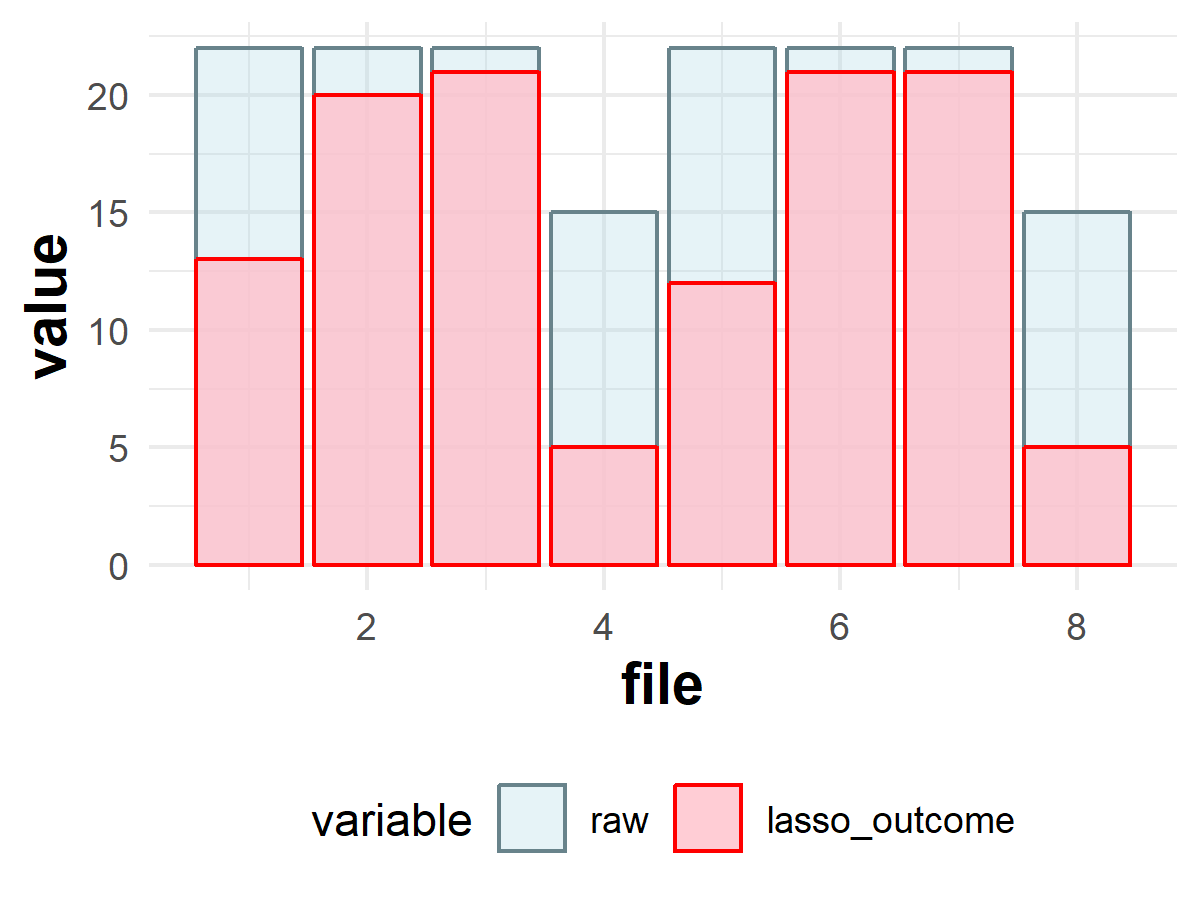
\includegraphics[width=\textwidth]{../plot/lasso_outcome.png}
    \caption{outcome (low)}
    %\label{fig:1}
  \end{subfigure}
  %
  \begin{subfigure}{0.24\textwidth}
    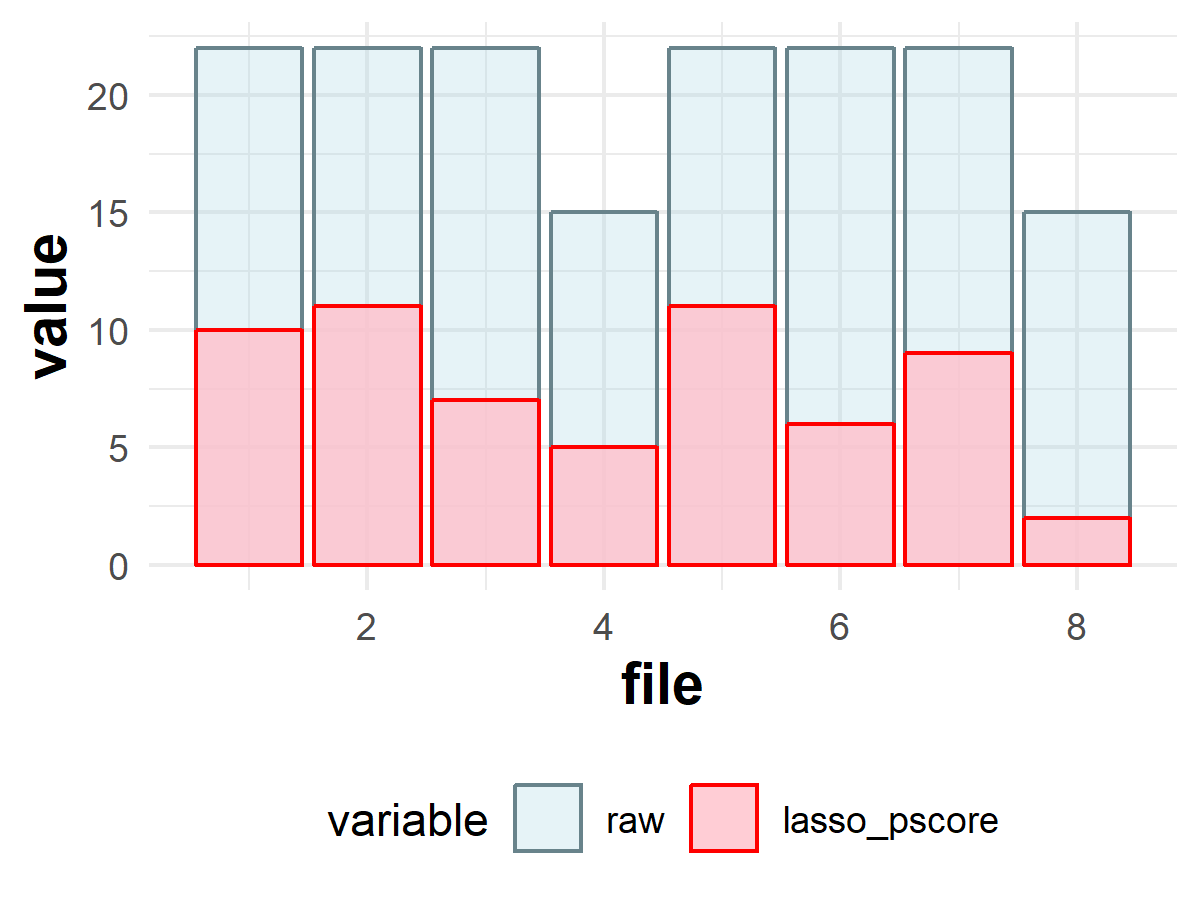
\includegraphics[width=\textwidth]{../plot/lasso_pscore.png}
    \caption{propensity score (low)}
    %\label{fig:2}
  \end{subfigure}
  \begin{subfigure}{0.24\textwidth}
    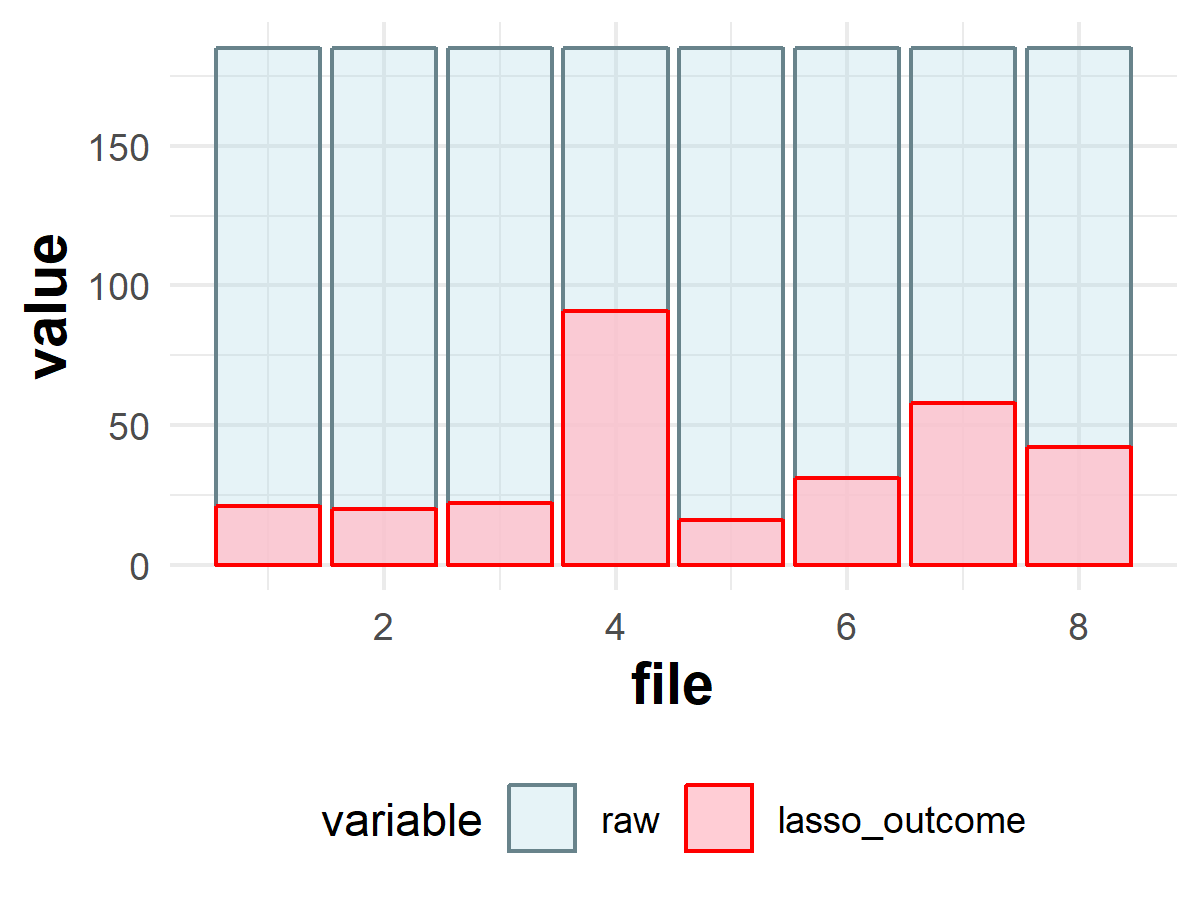
\includegraphics[width=\textwidth]{../plot/high_lasso_outcome.png}
    \caption{outcome (high)}
    %\label{fig:1}
  \end{subfigure}
  %
  \begin{subfigure}{0.24\textwidth}
    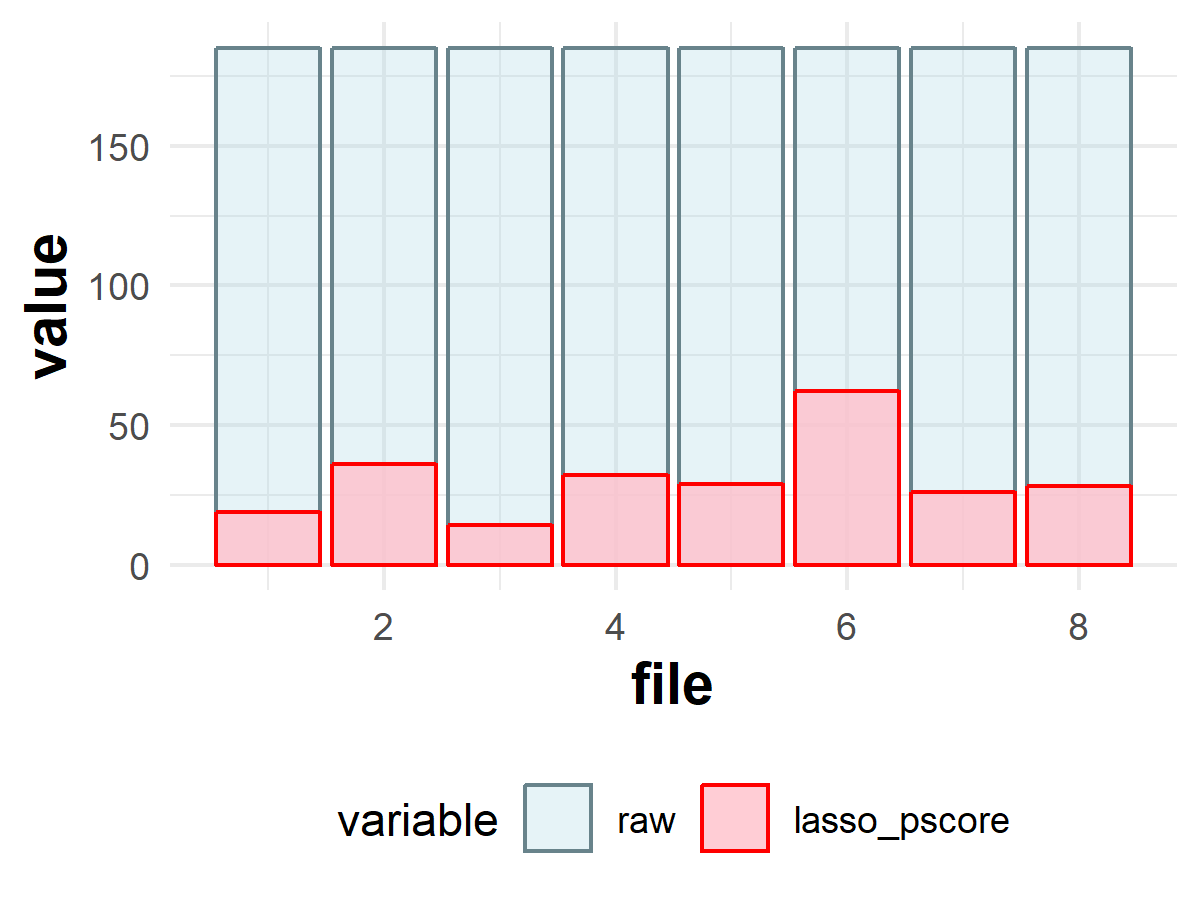
\includegraphics[width=\textwidth]{../plot/high_lasso_pscore.png}
    \caption{propensity score (high)}
    %\label{fig:2}
  \end{subfigure}
 \caption{Lasso selected variables for both data tracks} 
 \label{fig:lasso}
\end{figure}
Figure \ref{fig:lasso} shows the selected variables for the outcome model and propensity score model for both low dimension and high dimension track. We can see there are some non-significant features in the provided data set. The features selected will be carried along to the next modeling step.

\subsection{Causal Forest}
We also considered causal forest \cite{Athey2019} as another way to perform variable selection. For regular CART regression tree with samples $(V_i,Y_i)$, we start by recursively splitting the feature space until it's partitioned into a set of leaves $L$, each of which only contains a few training samples. Then, given a test point $v$, first identify which leaf $L(v)$ contain $v$, then prediction is: 
$$\hat{\mu}(v)=\frac{1}{|\{i:V_i \in L(v)\}|}\sum_{\{i:V_i \in L(v)\}}Y_i$$
Analogously, our dependent variables are $(Y_i,A_i)$, with ignorability, $\{Y_i(0),Y_i(1)\} \indep A_i | V_i$ ,and recall
$$\mbox{ATE}=E[E(\bY | \bA = 1, \bV) - E(\bY | \bA = 0, \bV)]$$
we have the causal forest predicted for ATE:
$$
\hat{ATE}(v) = \frac{1}{|\{i:A_i=1, V_i \in L\}|}\sum_{\{i:A_i=1, V_i \in L(v)\}} Y_i - \frac{1}{|\{i:A_i=0, V_i \in L\}|}\sum_{\{i:A_i=0, V_i \in L(v)\}} Y_i
$$
The authors show the estimate is point wise consistent: $\hat{\tau} \rightarrow \tau \mbox{ in Probability}$, and have an asymptotically Gaussian and centered sampling distribution: $(\hat{\tau}-\tau)/\sqrt{Var(\hat{\tau})} \rightarrow \mathcal{N}(0,1)$. Similar to before, we will show results for directly apply causal forest, and apply the two stage causal forest algorithm. For two stage, firstly fit the separate regression/classification tree for the outcome and treatment, then use selected variable from those trees to build a new causal tree to estimate ATE.
\section{Result}\label{sec:result}
\subsection{Training dataset}
Firstly, we show the results of all basic methods and the two-step methods for low dimensional data in Figure \ref{fig:twosteplow}. Considering the big difference between total number of variables and the number of selected variables in high dimension track, the comparison is also shown in \ref{fig:twostephigh}.
\begin{figure}[h]
  \begin{subfigure}{0.24\textwidth}
    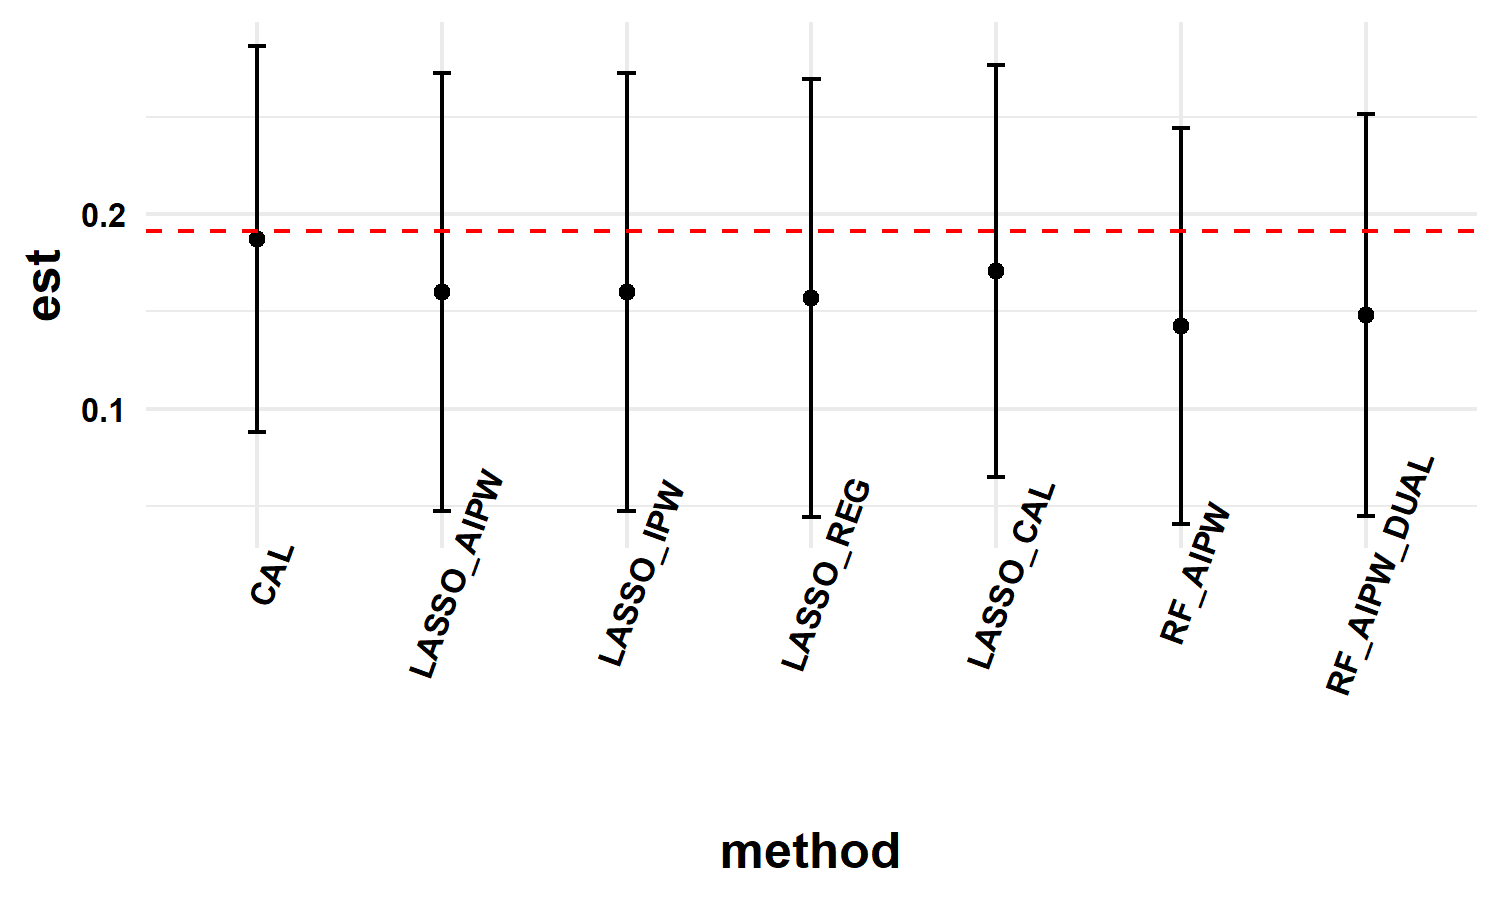
\includegraphics[width=\textwidth]{../plot/method_comparison_1.png}
    \caption{test file 1}
    %\label{fig:1}
  \end{subfigure}
  %
  \begin{subfigure}{0.24\textwidth}
    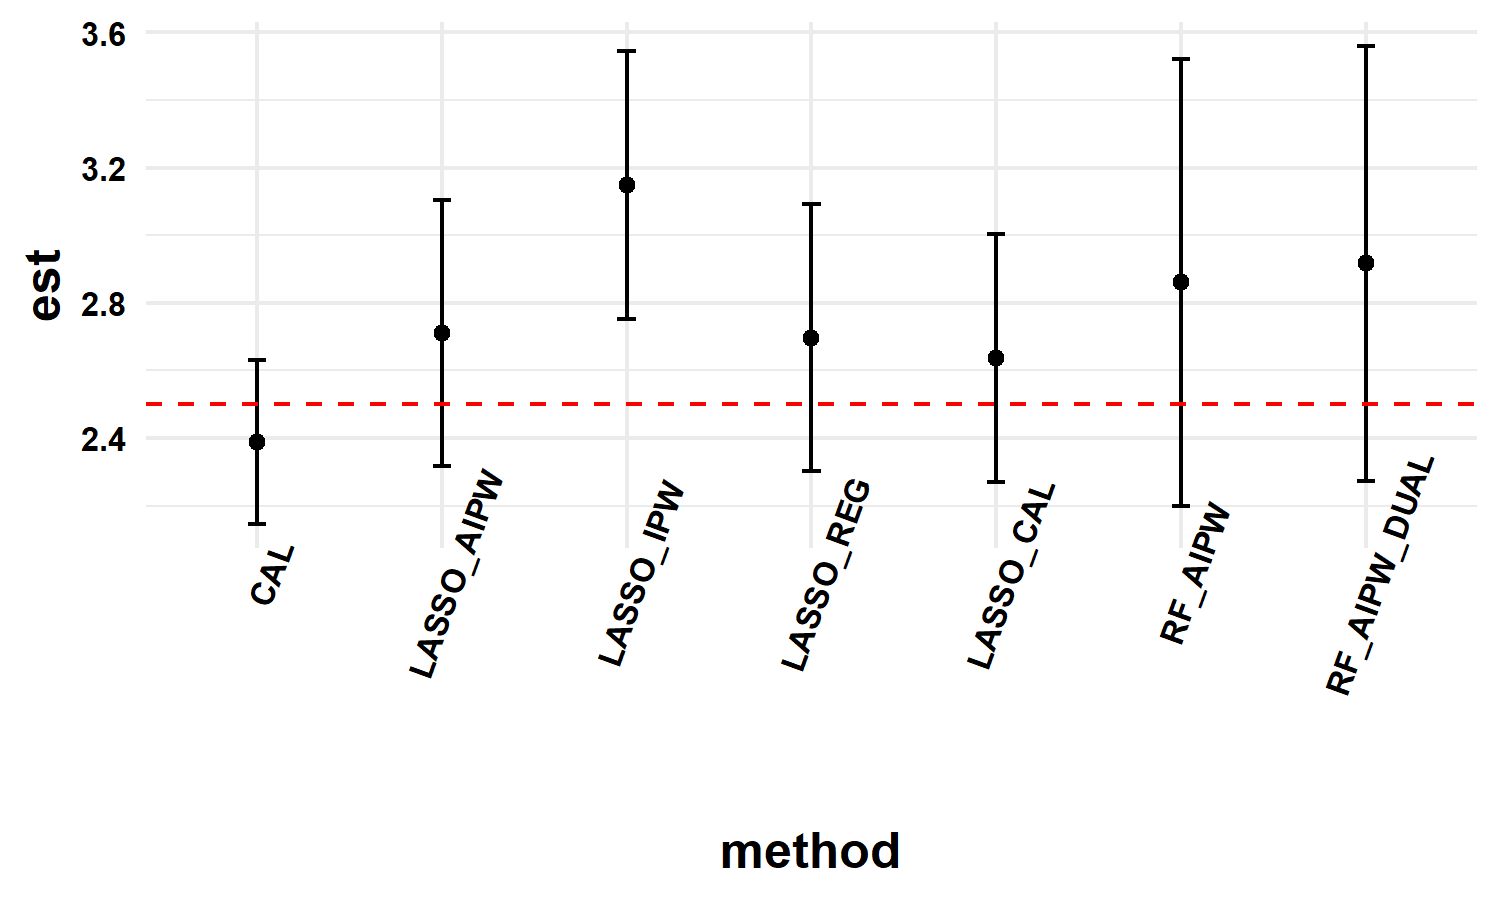
\includegraphics[width=\textwidth]{../plot/method_comparison_2.png}
    \caption{test file 2}
    %\label{fig:2}
  \end{subfigure}
  \begin{subfigure}{0.24\textwidth}
    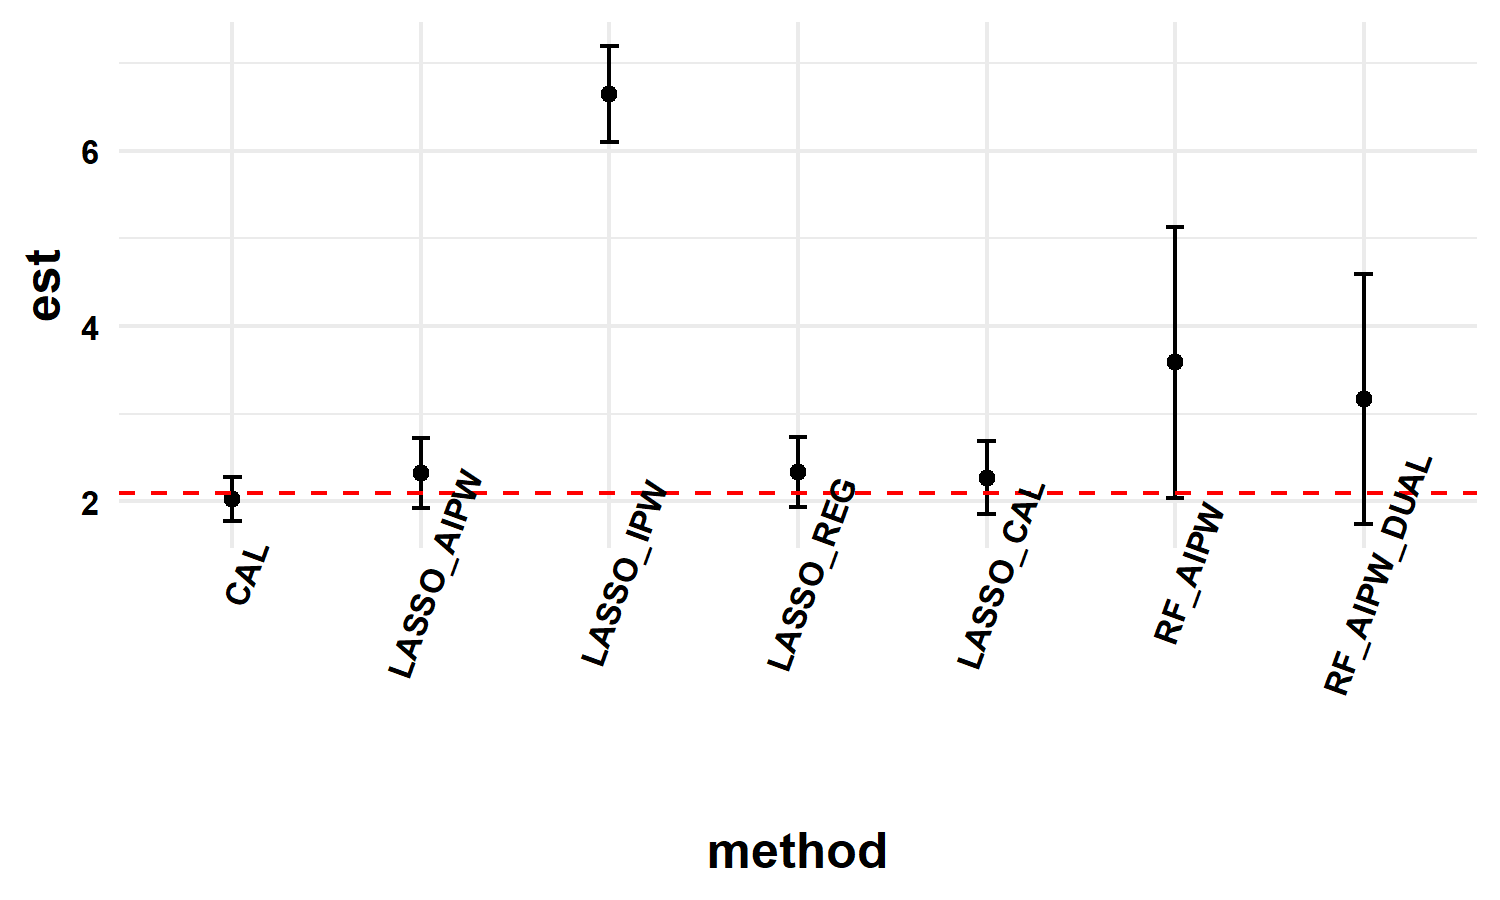
\includegraphics[width=\textwidth]{../plot/method_comparison_3.png}
    \caption{test file 3}
    %\label{fig:1}
  \end{subfigure}
  %
  \begin{subfigure}{0.24\textwidth}
    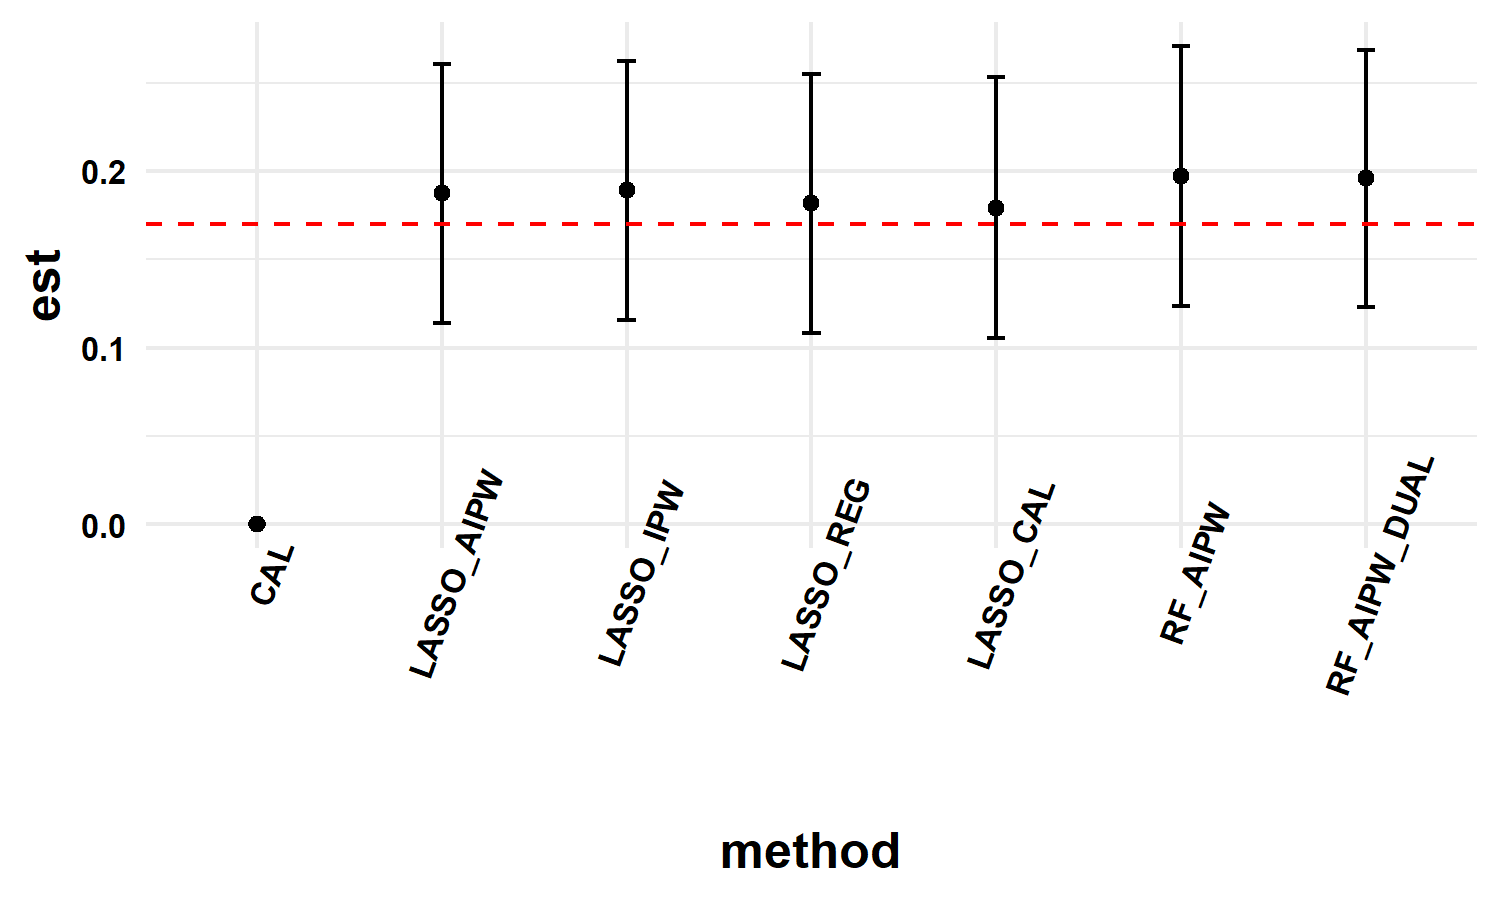
\includegraphics[width=\textwidth]{../plot/method_comparison_4.png}
    \caption{test file 4}
    %\label{fig:2}
  \end{subfigure}
  \begin{subfigure}{0.24\textwidth}
    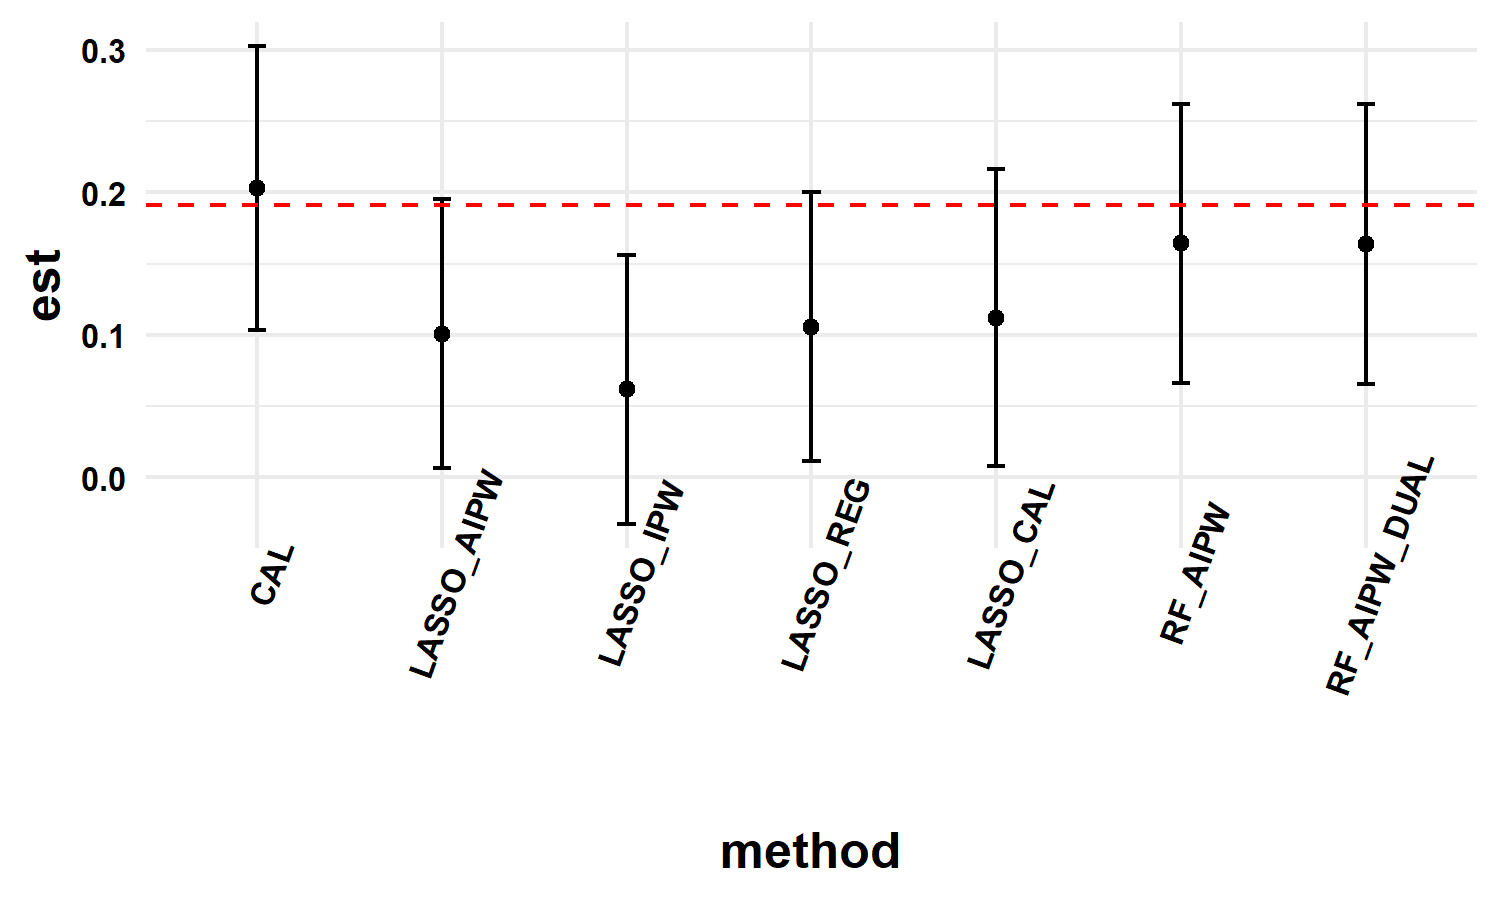
\includegraphics[width=\textwidth]{../plot/method_comparison_5.png}
    \caption{test file 5}
    %\label{fig:1}
  \end{subfigure}
  %
  \begin{subfigure}{0.24\textwidth}
    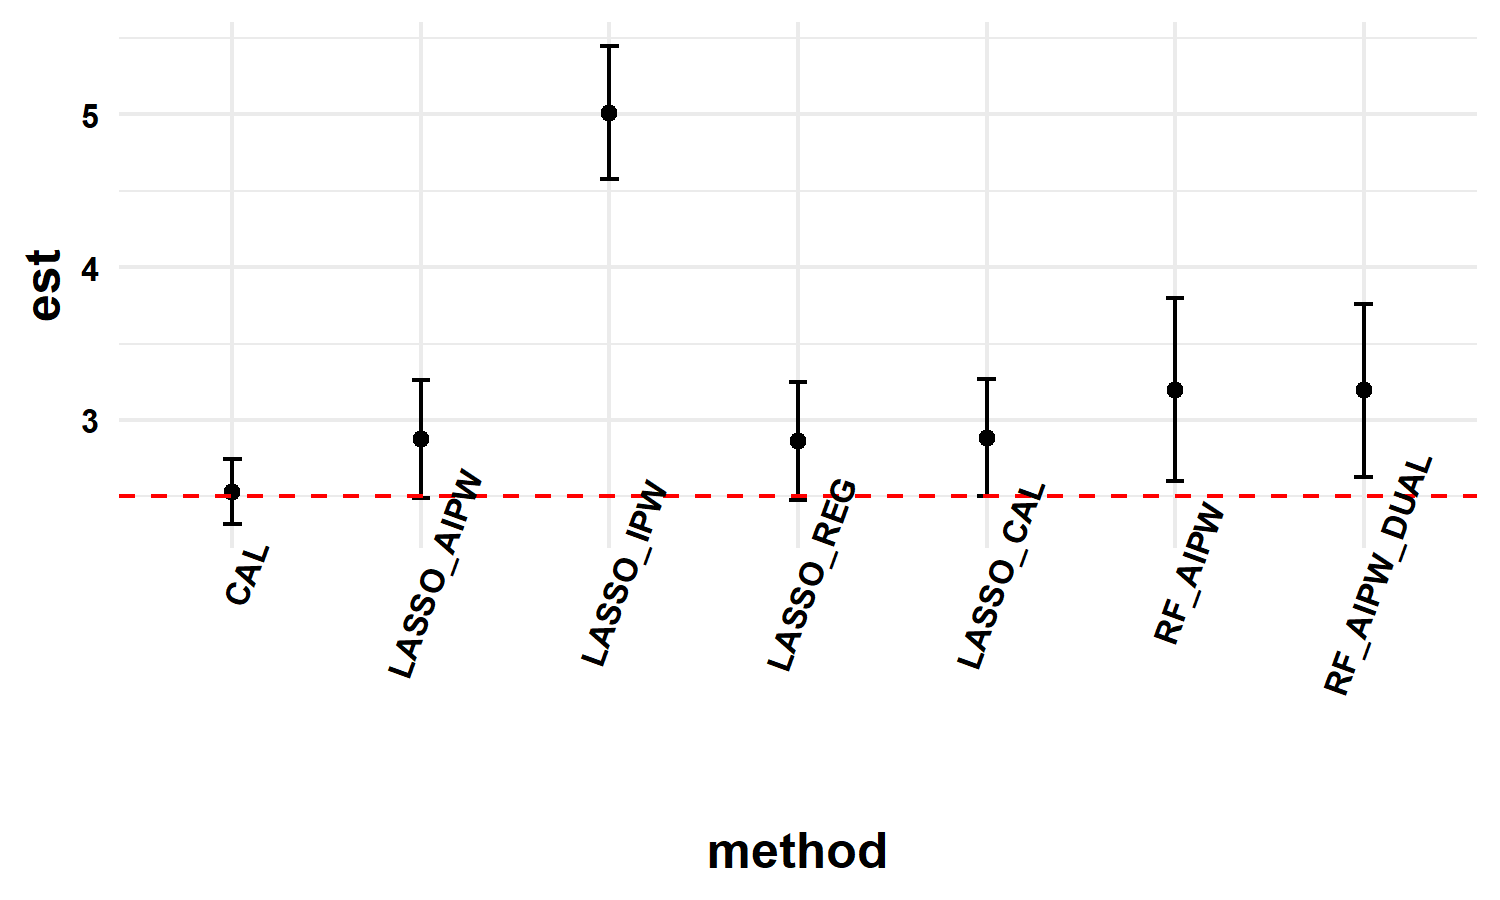
\includegraphics[width=\textwidth]{../plot/method_comparison_6.png}
    \caption{test file 6}
    %\label{fig:2}
  \end{subfigure}
  \begin{subfigure}{0.24\textwidth}
    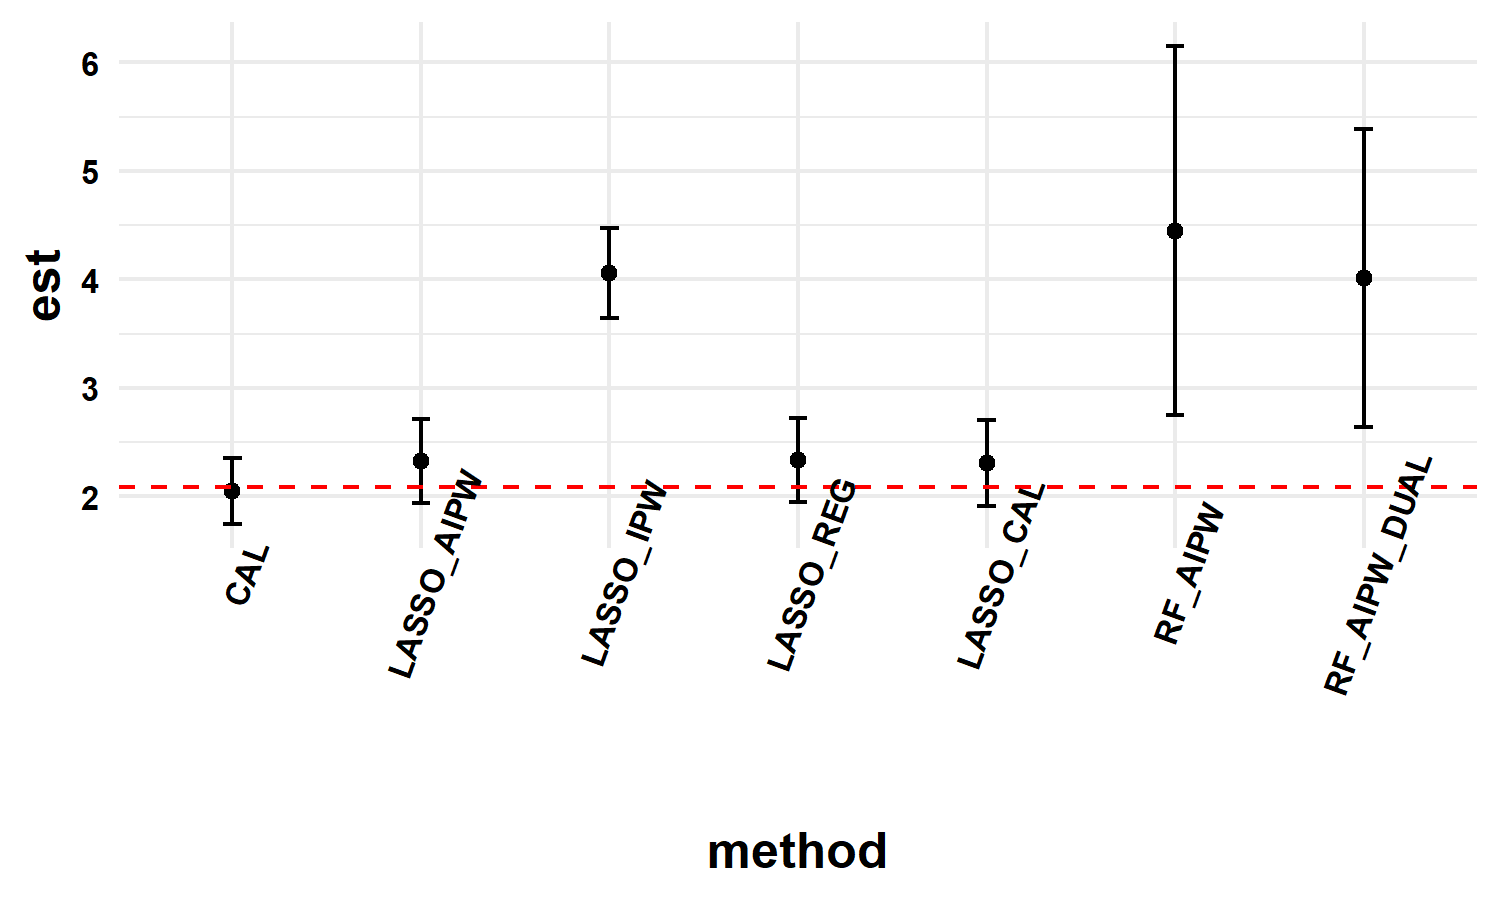
\includegraphics[width=\textwidth]{../plot/method_comparison_7.png}
    \caption{test file 7}
    %\label{fig:1}
  \end{subfigure}
  %
  \begin{subfigure}{0.24\textwidth}
    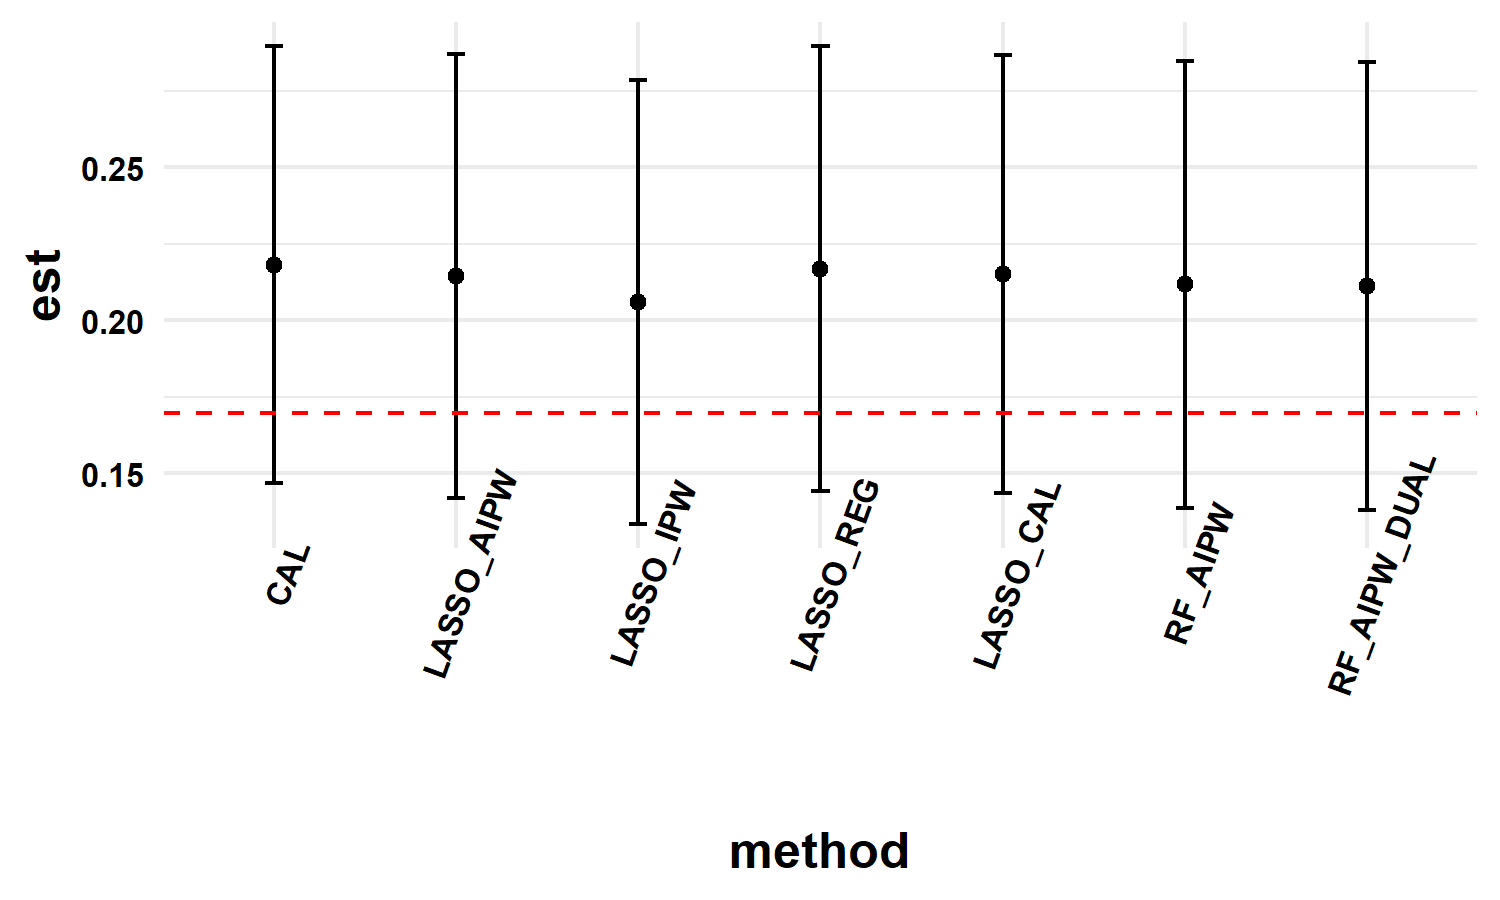
\includegraphics[width=\textwidth]{../plot/method_comparison_8.png}
    \caption{test file 8}
    %\label{fig:2}
  \end{subfigure}
  \caption{Estimation of ATE with 95\% confidence interval on the low track files} 
  \label{fig:twosteplow}
\end{figure}
From the low dimension track, we can see the two step IPW is quite unstable, which matches our prediction given it failed to consider the propensity score part. Similar conclusion holds for high dimension track as well. 
\begin{figure}[h]
  \begin{subfigure}{0.24\textwidth}
    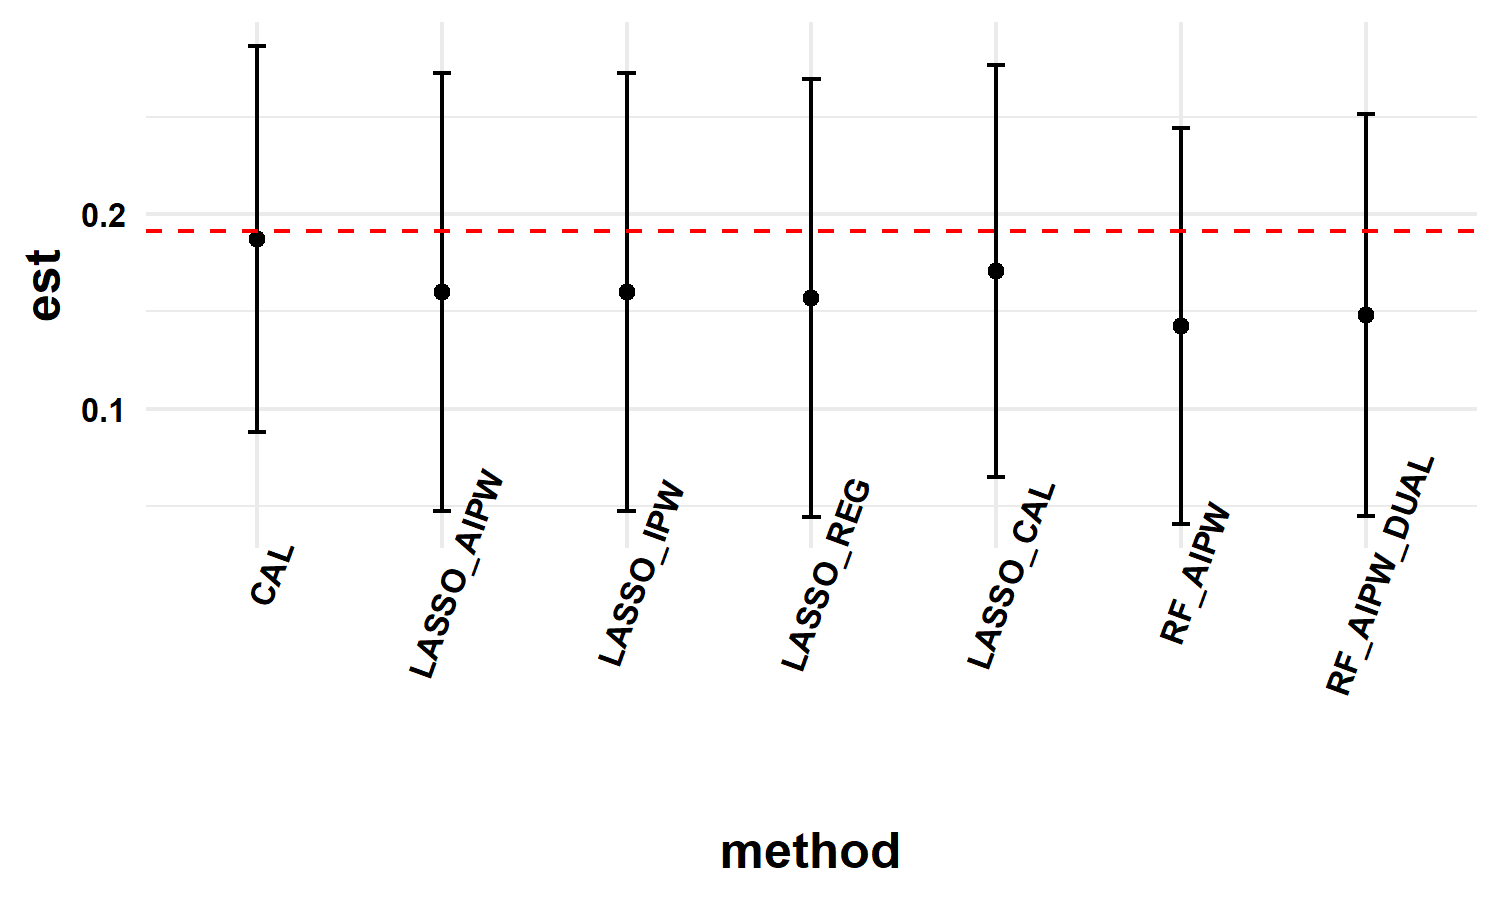
\includegraphics[width=\textwidth]{../plot/method_comparison_high_1.png}
    \caption{test file 1}
    %\label{fig:1}
  \end{subfigure}
  %
  \begin{subfigure}{0.24\textwidth}
    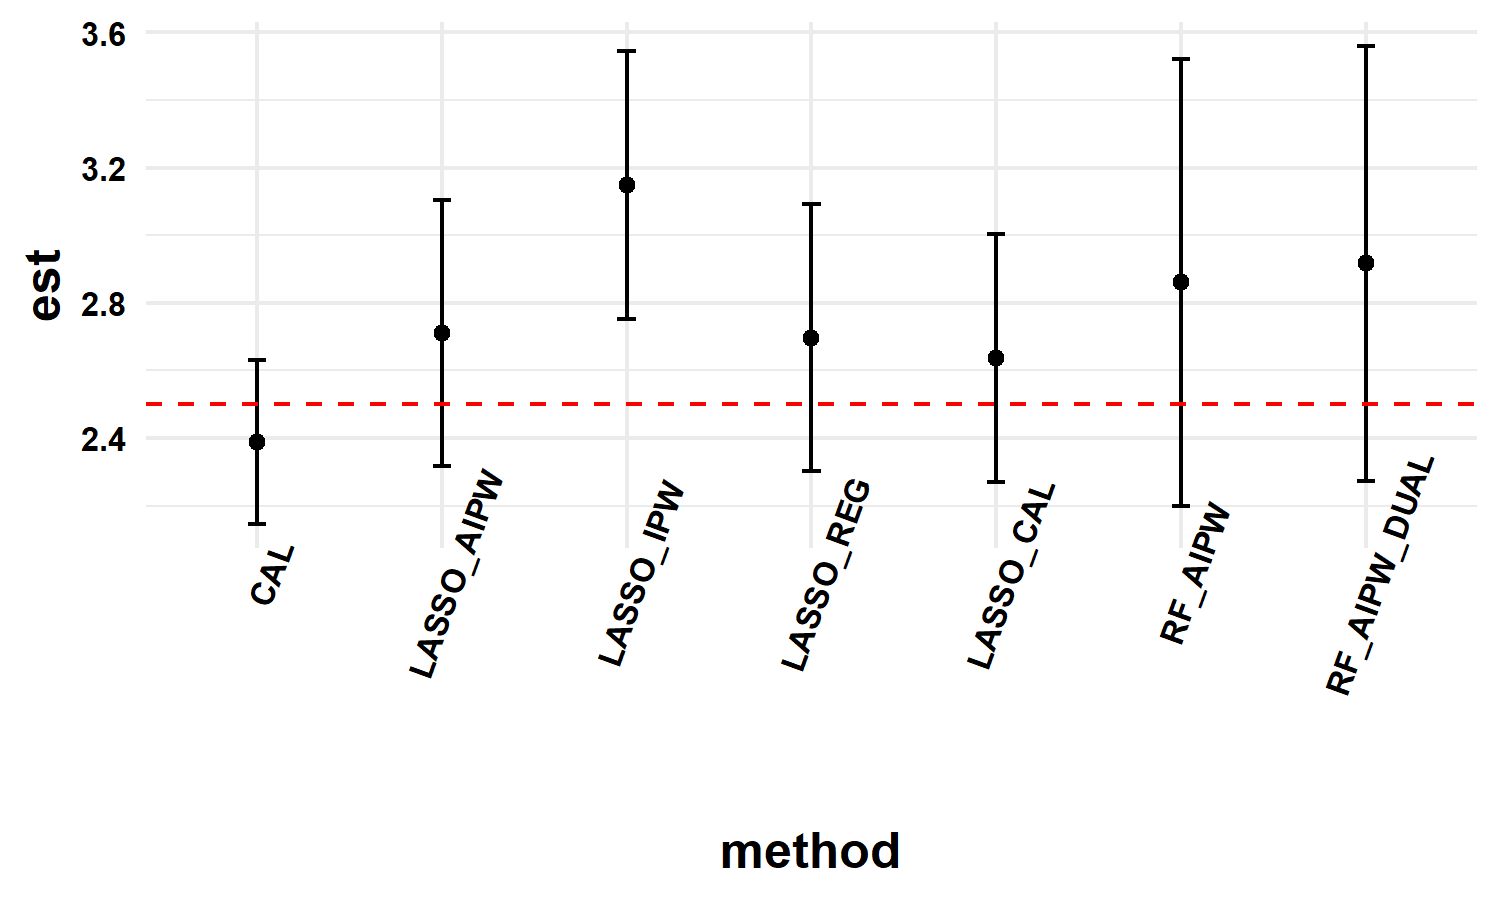
\includegraphics[width=\textwidth]{../plot/method_comparison_high_2.png}
    \caption{test file 2}
    %\label{fig:2}
  \end{subfigure}
  \begin{subfigure}{0.24\textwidth}
    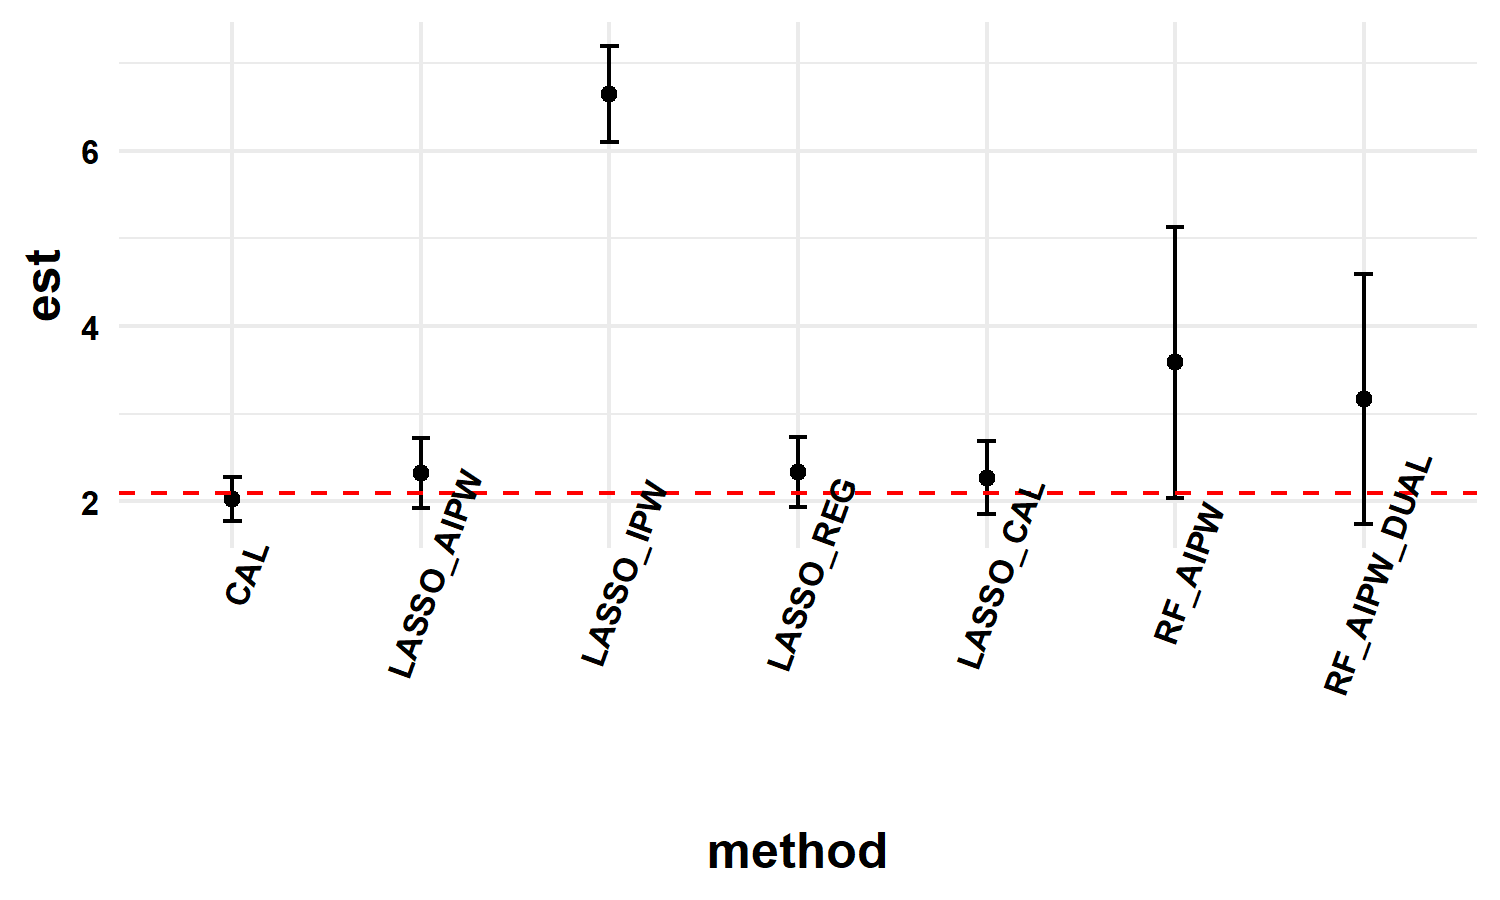
\includegraphics[width=\textwidth]{../plot/method_comparison_high_3.png}
    \caption{test file 3}
    %\label{fig:1}
  \end{subfigure}
  %
  \begin{subfigure}{0.24\textwidth}
    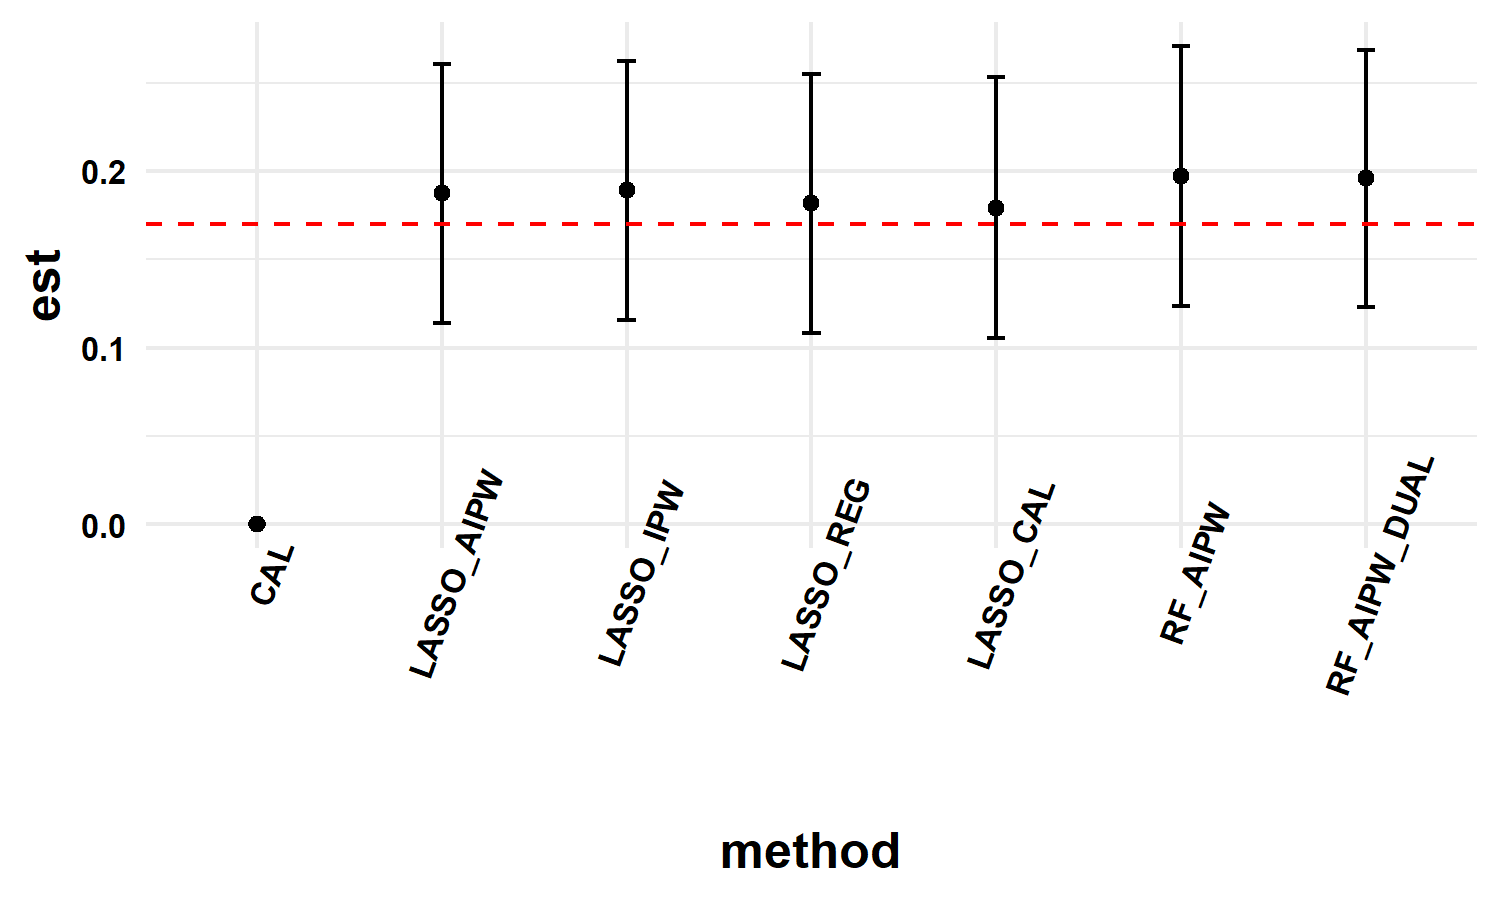
\includegraphics[width=\textwidth]{../plot/method_comparison_high_4.png}
    \caption{test file 4}
    %\label{fig:2}
  \end{subfigure}
    \begin{subfigure}{0.24\textwidth}
    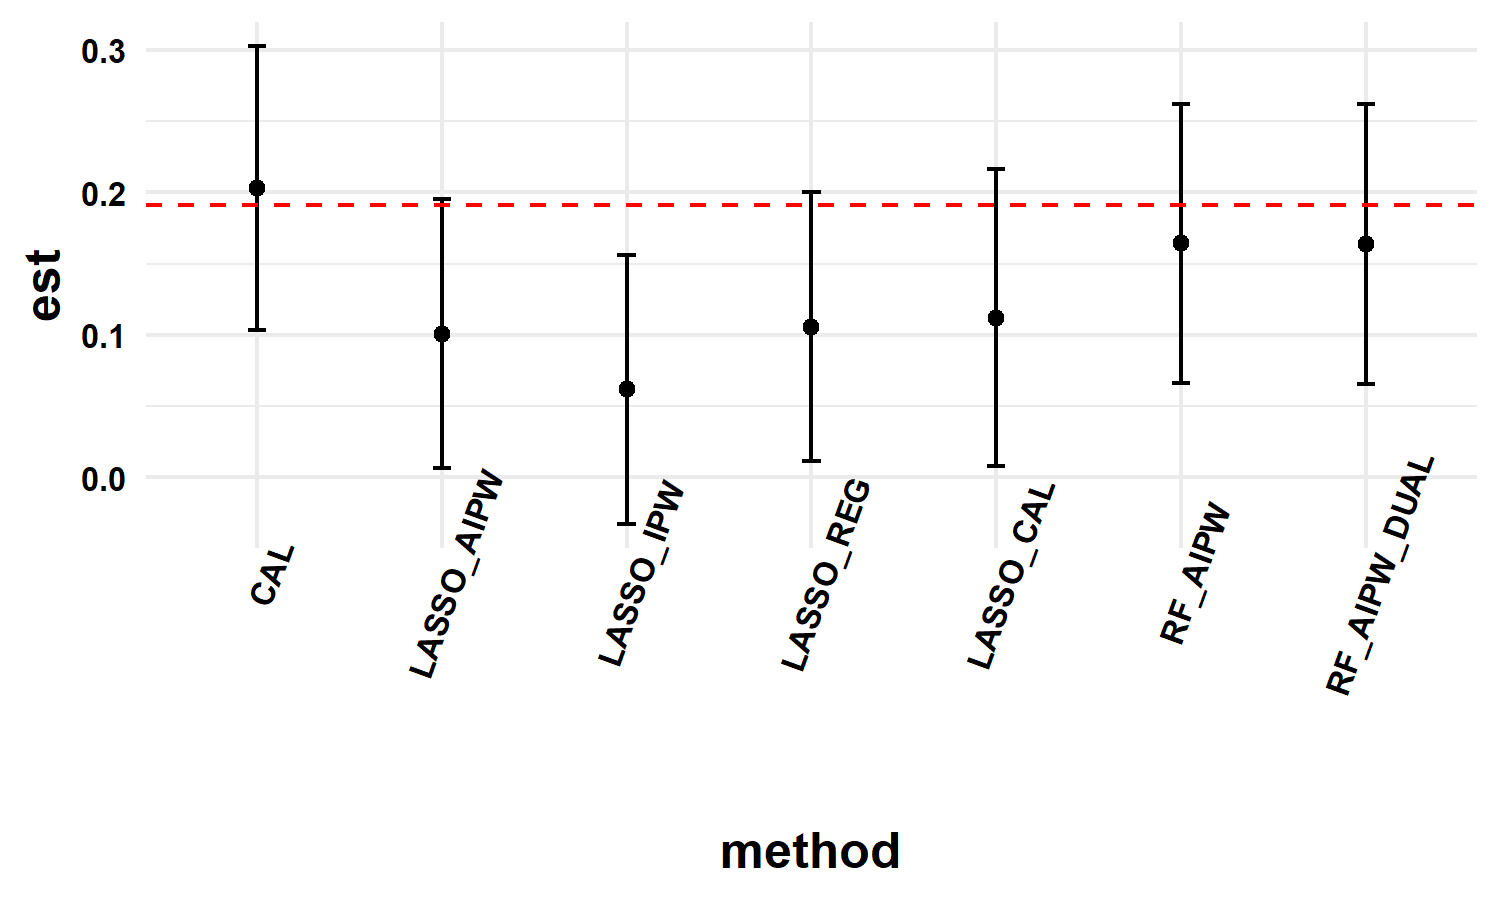
\includegraphics[width=\textwidth]{../plot/method_comparison_high_5.png}
    \caption{test file 5}
    %\label{fig:1}
  \end{subfigure}
  %
  \begin{subfigure}{0.24\textwidth}
    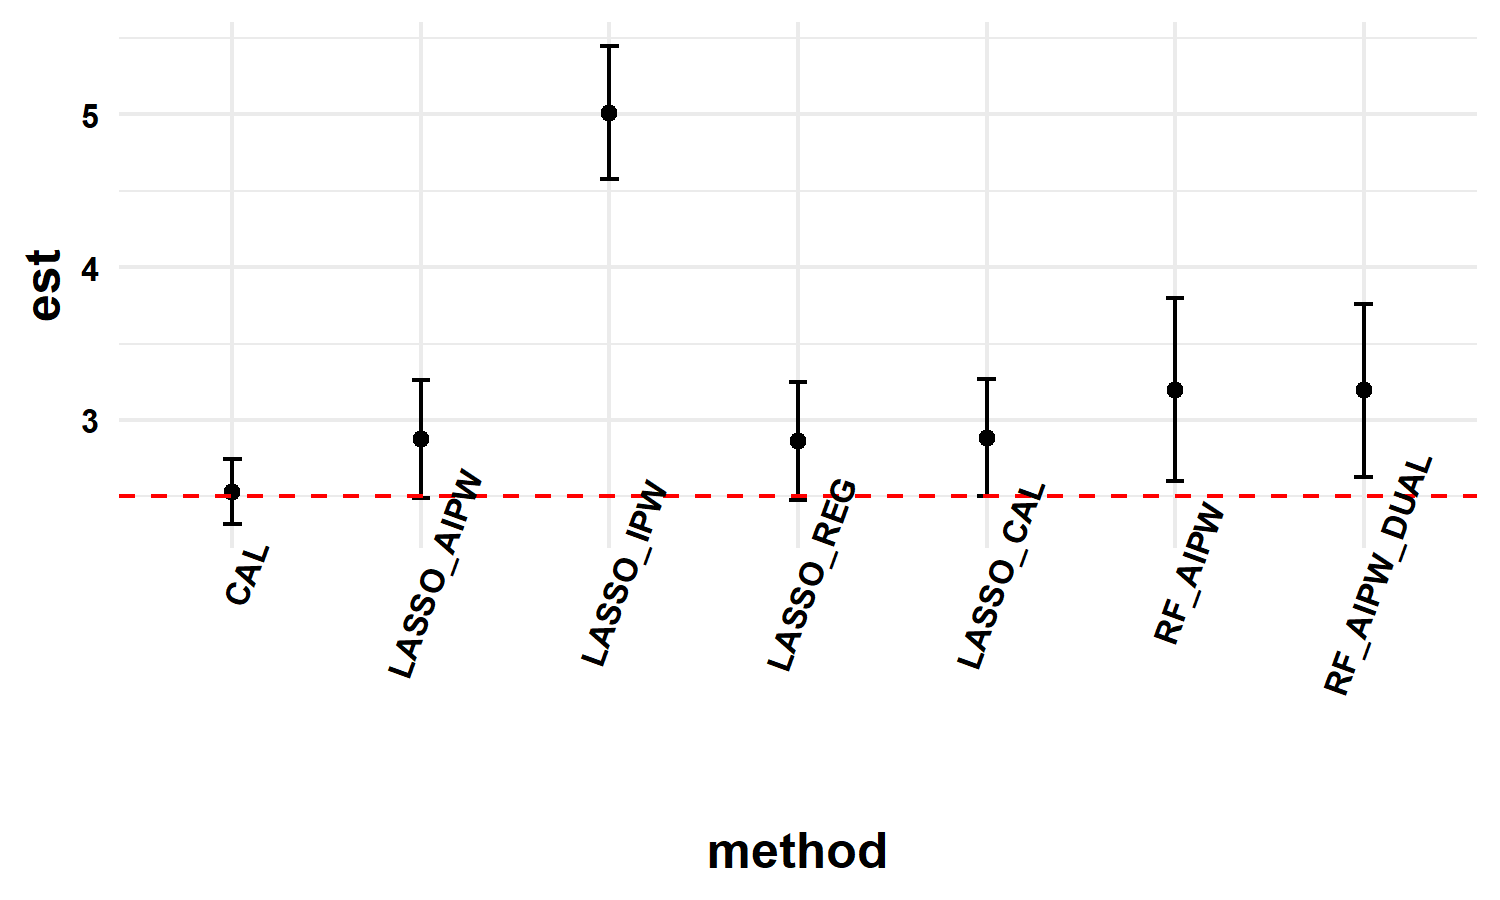
\includegraphics[width=\textwidth]{../plot/method_comparison_high_6.png}
    \caption{test file 6}
    %\label{fig:2}
  \end{subfigure}
  \begin{subfigure}{0.24\textwidth}
    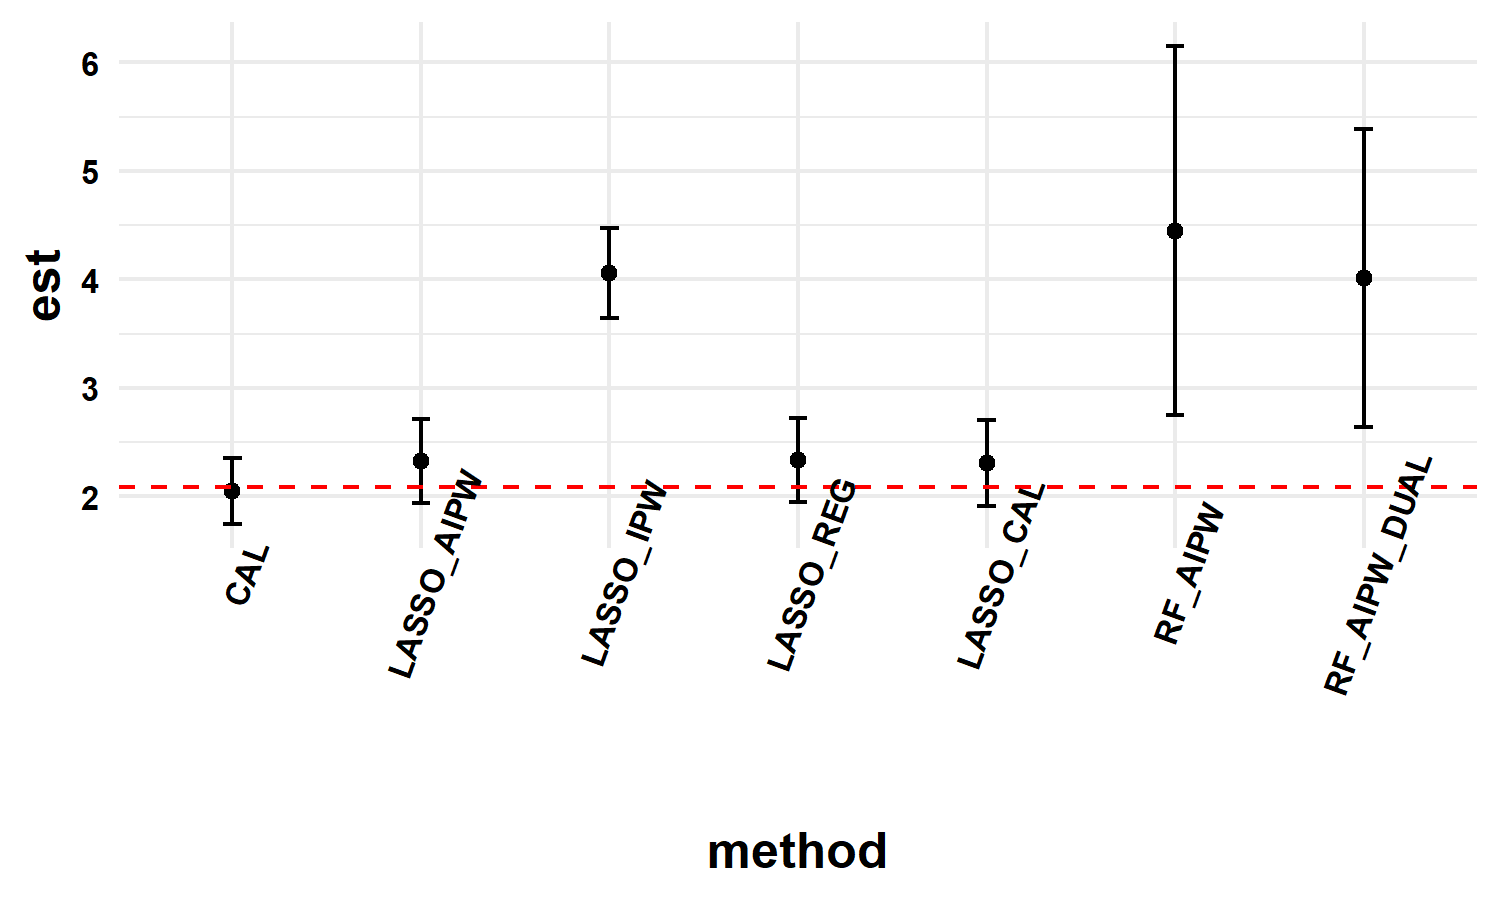
\includegraphics[width=\textwidth]{../plot/method_comparison_high_7.png}
    \caption{test file 7}
    %\label{fig:1}
  \end{subfigure}
  %
  \begin{subfigure}{0.24\textwidth}
    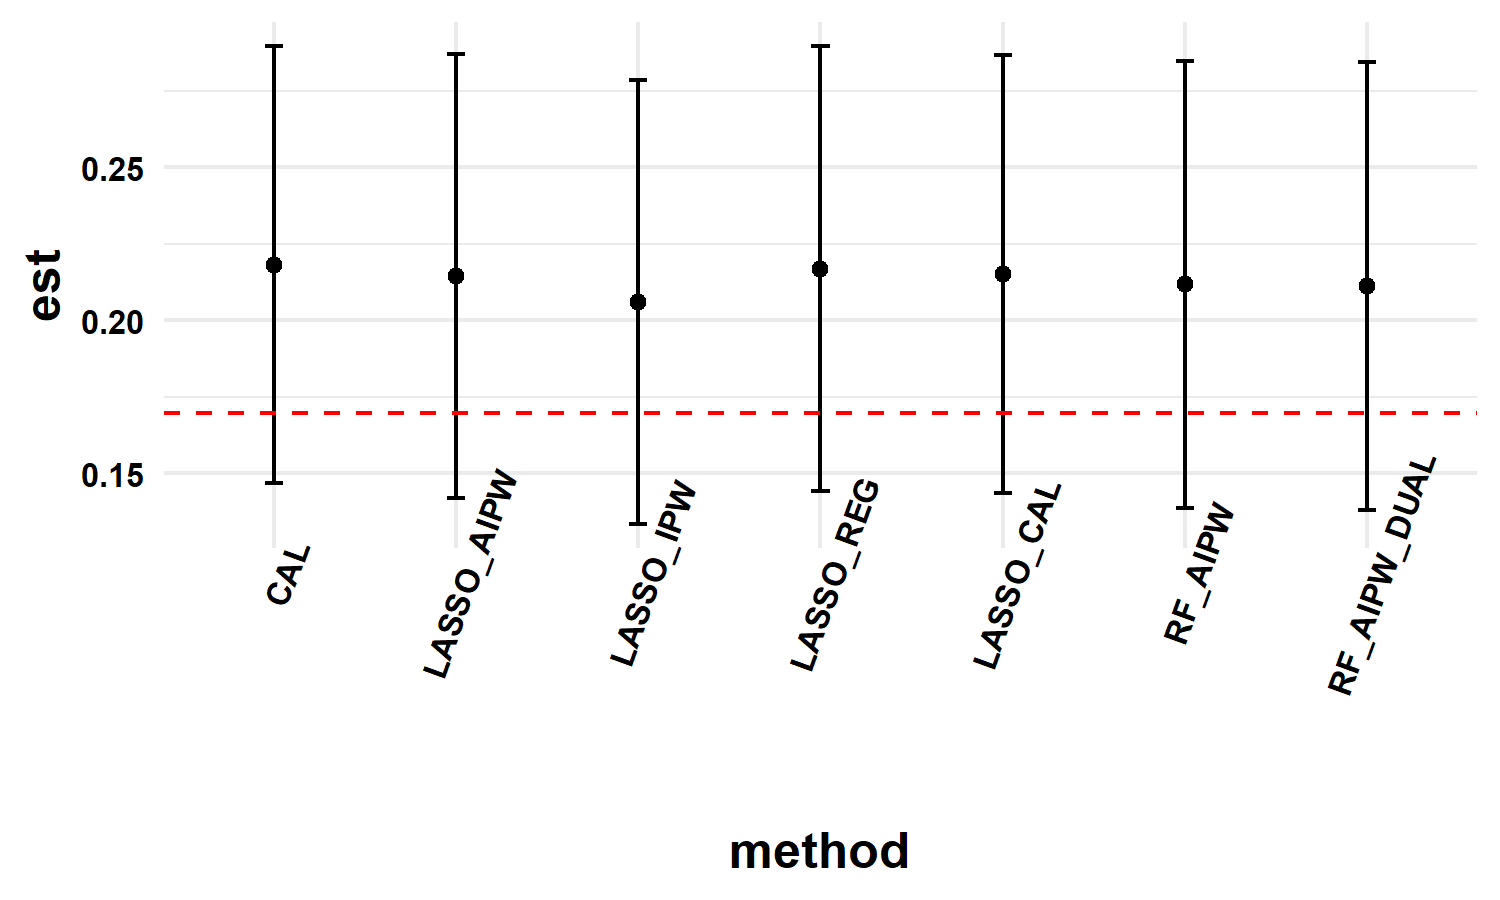
\includegraphics[width=\textwidth]{../plot/method_comparison_high_8.png}
    \caption{test file 8}
    %\label{fig:2}
  \end{subfigure}
 \caption{Estimation of ATE with 95\% confidence interval on the files of high track} 
\label{fig:twostephigh}
\end{figure}
Table \ref{tab:summarylow} is a summary for Figure \ref{fig:twosteplow}. Y indicates the true ATE is contained in the 95\% confidence interval of that specific method, the annotated N indicates the method fail to capture true ATE. We can see the non-parametric estimation CAL and the two step causal forest with AIPW formula performs best.  
\begin{table}[h]
%\begin{minipage}{\textwidth}
  \begin{minipage}{0.44\textwidth}
    \centering

\label{tab:summarylow}
\scalebox{0.65}{
\begin{tabular}{@{}cccccccc@{}}
\toprule
\multirow{2}{*}{} & \multirow{2}{*}{CAL} & \multirow{2}{*}{\begin{tabular}[c]{@{}c@{}}LASSO\\ AIPW\end{tabular}} & \multirow{2}{*}{\begin{tabular}[c]{@{}c@{}}LASSO\\ IPW\end{tabular}} & \multirow{2}{*}{\begin{tabular}[c]{@{}c@{}}LASSO\\ REG\end{tabular}} & \multirow{2}{*}{\begin{tabular}[c]{@{}c@{}}LASSO\\ CAL\end{tabular}} & \multirow{2}{*}{\begin{tabular}[c]{@{}c@{}}RF\\ AIPW\end{tabular}} & \multirow{2}{*}{\begin{tabular}[c]{@{}c@{}}RF\_AIPW\\ DUAL\end{tabular}} \\
                  &                      &                                                                       &                                                                      &                                                                      &                                                                      &                                                                    &                                                                          \\ \midrule
1                 & Y                    & Y                                                                     & Y                                                                    & Y                                                                    & Y                                                                    & Y                                                                  & Y                                                                        \\
2                 & Y                    & Y                                                                     & N*                                                                   & Y                                                                    & Y                                                                    & Y                                                                  & Y                                                                        \\
3                 & Y                    & Y                                                                     & N*                                                                   & Y                                                                    & Y                                                                    & N*                                                                 & Y                                                                        \\
4                 & N*                    & Y                                                                     & Y                                                                    & Y                                                                    & Y                                                                    & Y                                                                  & Y                                                                        \\
5                 & Y                    & N*                                                                    & N*                                                                    & Y                                                                    & Y                                                                    & Y                                                                  & Y                                                                        \\
6                 & Y                    & Y                                                                     & N*                                                                   & Y                                                                    & Y                                                                    & N*                                                              & N*                                                                      \\
7                 & Y                    & Y                                                                     & N*                                                                   & Y                                                                    & Y                                                                    & N*                                                                 & N*                                                                       \\
8                 & Y                    & Y                                                                     & Y                                                                    & Y                                                                    & Y                                                                    & Y                                                                  & Y                                                                        \\ \bottomrule
\end{tabular}}
    \captionof{table}{Summary table of 95\% confidence interval for all methods}
\end{minipage}
  \hfill
  \begin{minipage}{0.50\textwidth}
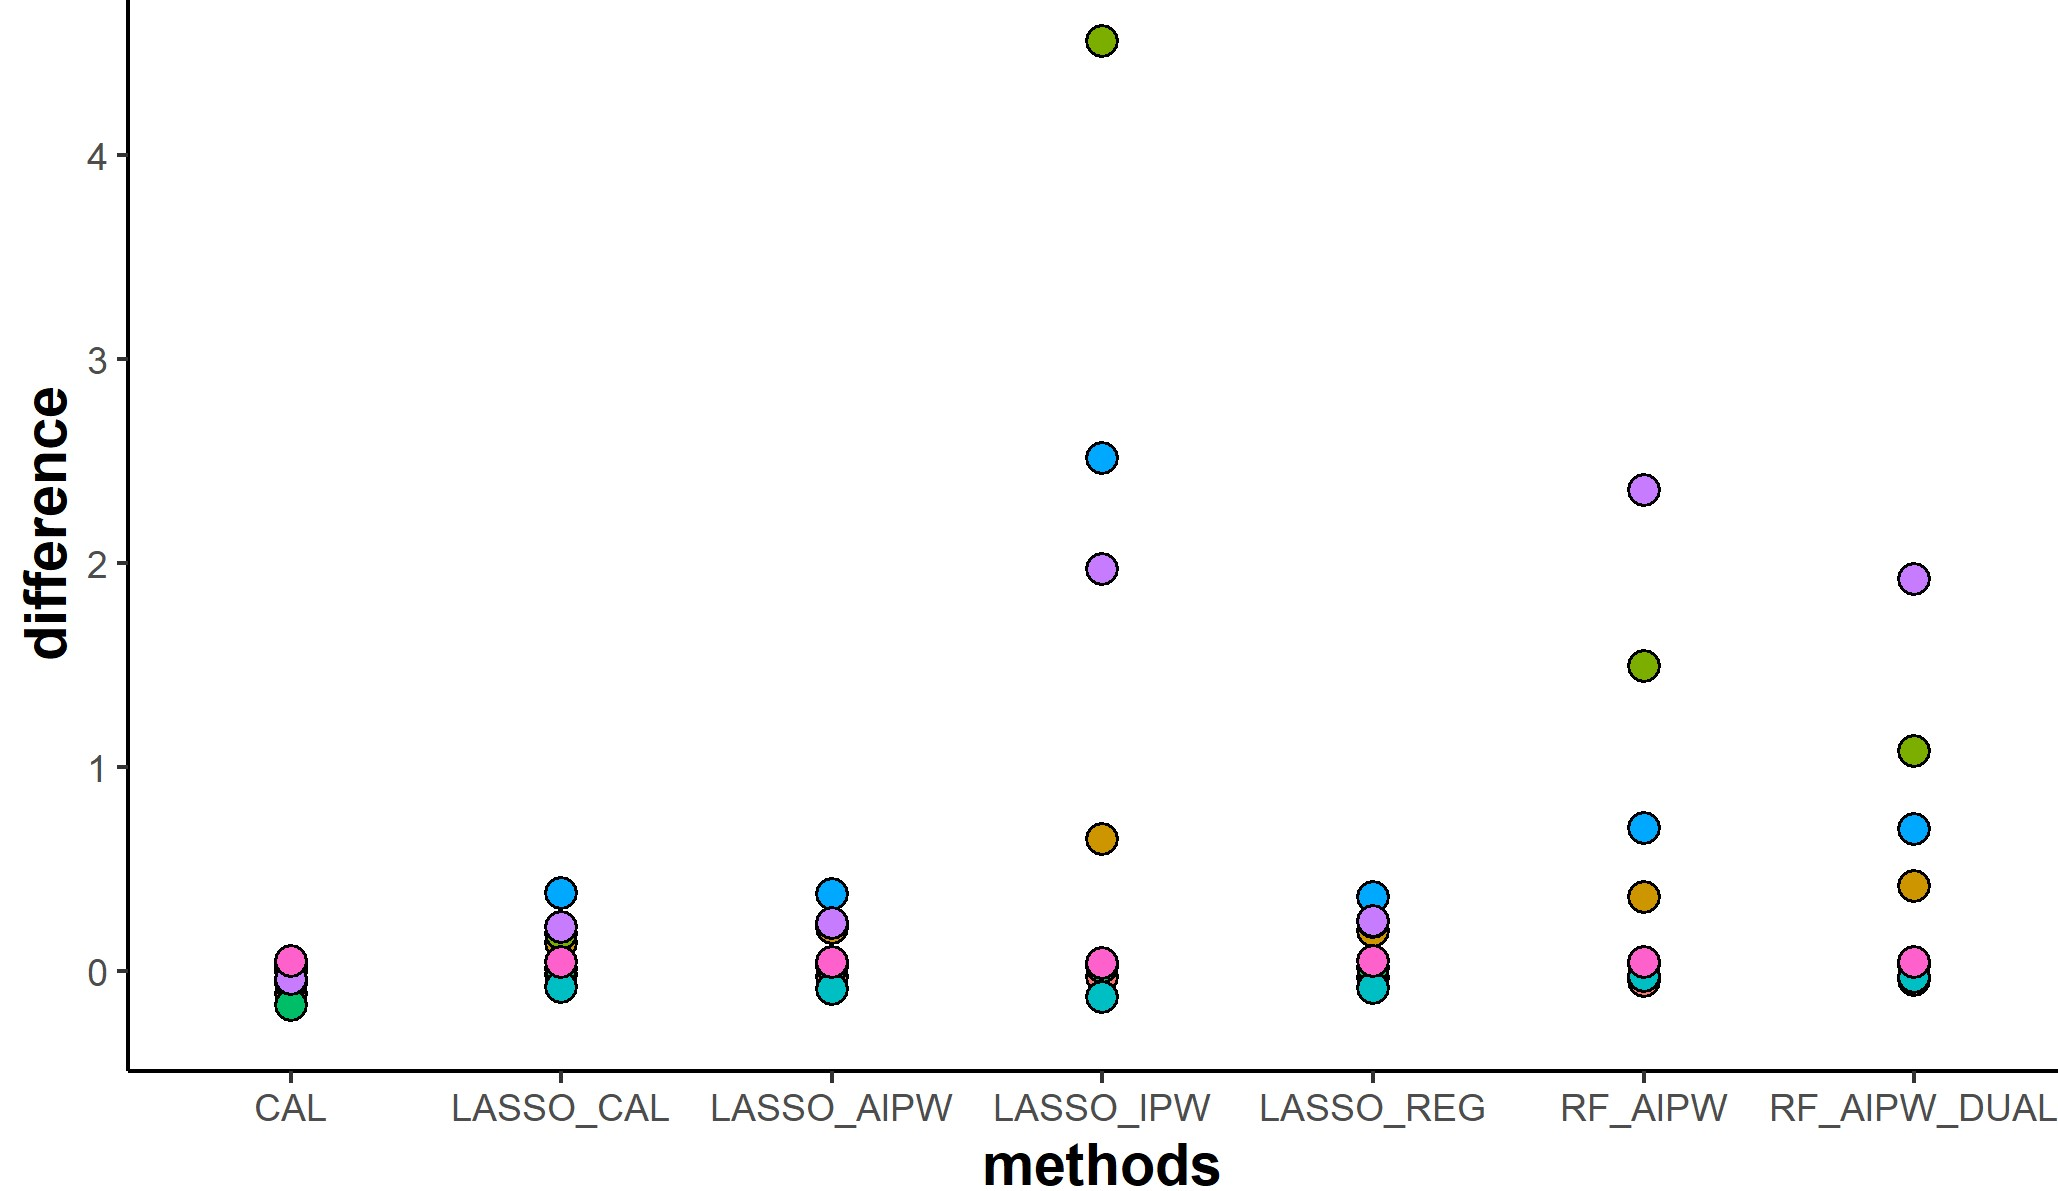
\includegraphics[width=1\textwidth, height=4cm]{../plot/comparison_diffcut.jpg}
    \captionof{figure}{Comparison of the difference with true ATE for all methods}
    \label{fig:pointdifflow}
   \end{minipage}
\end{table}
Aside from the TRUE/FALSE answer of whether the true ATE is included in the 95\% confidence interval, the actual difference of point estimate and true ATE is also of our interest. The results of differences between True ATE and point estimate based on all 8 methods are presented in Figure \ref{fig:pointdifflow}. We can see LASSO\_IPW have largest differences compare to other methods, which confirms the previous conclusion that LASSO\_IPW fails to calculate the ATE. Another interesting thing is that even the causal forest methods contain the true ATE in most cases, it also have fairly large point estimate difference in some cases, which can be explained by the large covariance induced in the method. 

\subsection{Test dataset}
We perform the above methods on all 3,200 testing files. Since there is no true ATE to compare to, and all we do have the information that those files are generated from 32 separate DPGs and each DGP have the same type ATE. In other words, there should be at most 32 unique true ATEs, thus one way to check the quality of the results for test dataset is to cluster the estimated ATE, hopefully we can see a clear division. 

Figure \ref{fig:cluster1} is the result from K-means clustering with pre-specified 32 clusters. We can see that it's not easy to tell if the result makes sense, similarly for the univariate clustering methods as shown in Figure \ref{fig:cluster2}.
\begin{figure}[H]
\centering
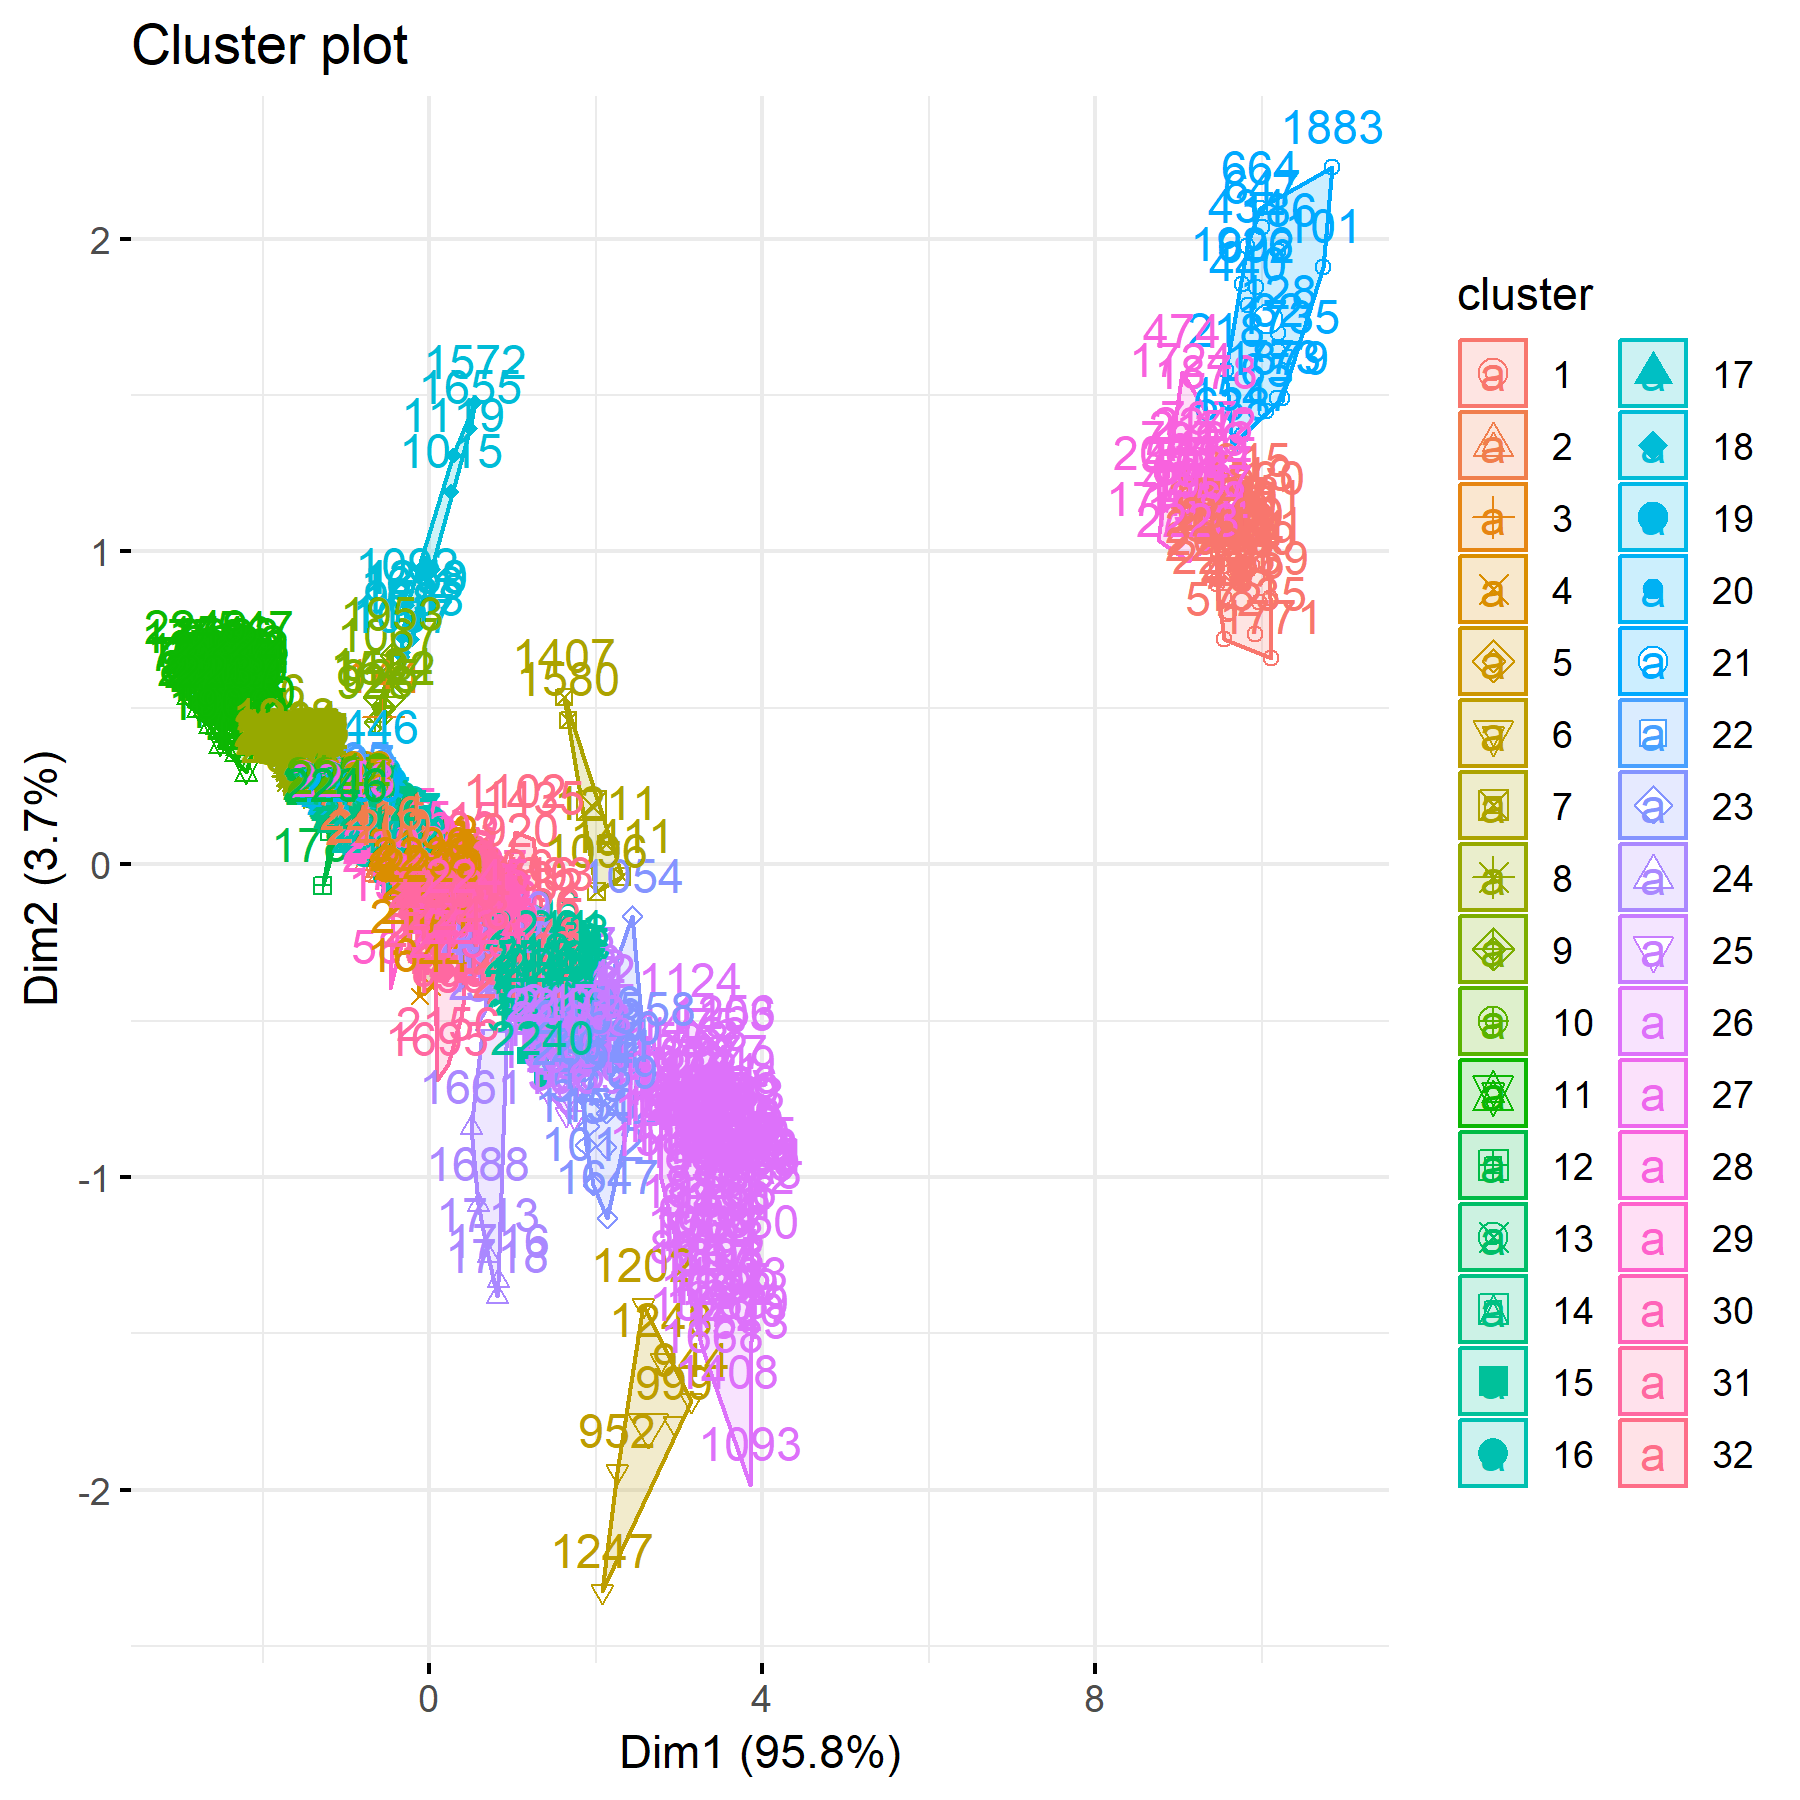
\includegraphics[width=0.48\textwidth]{../plot/cluster_full.png}
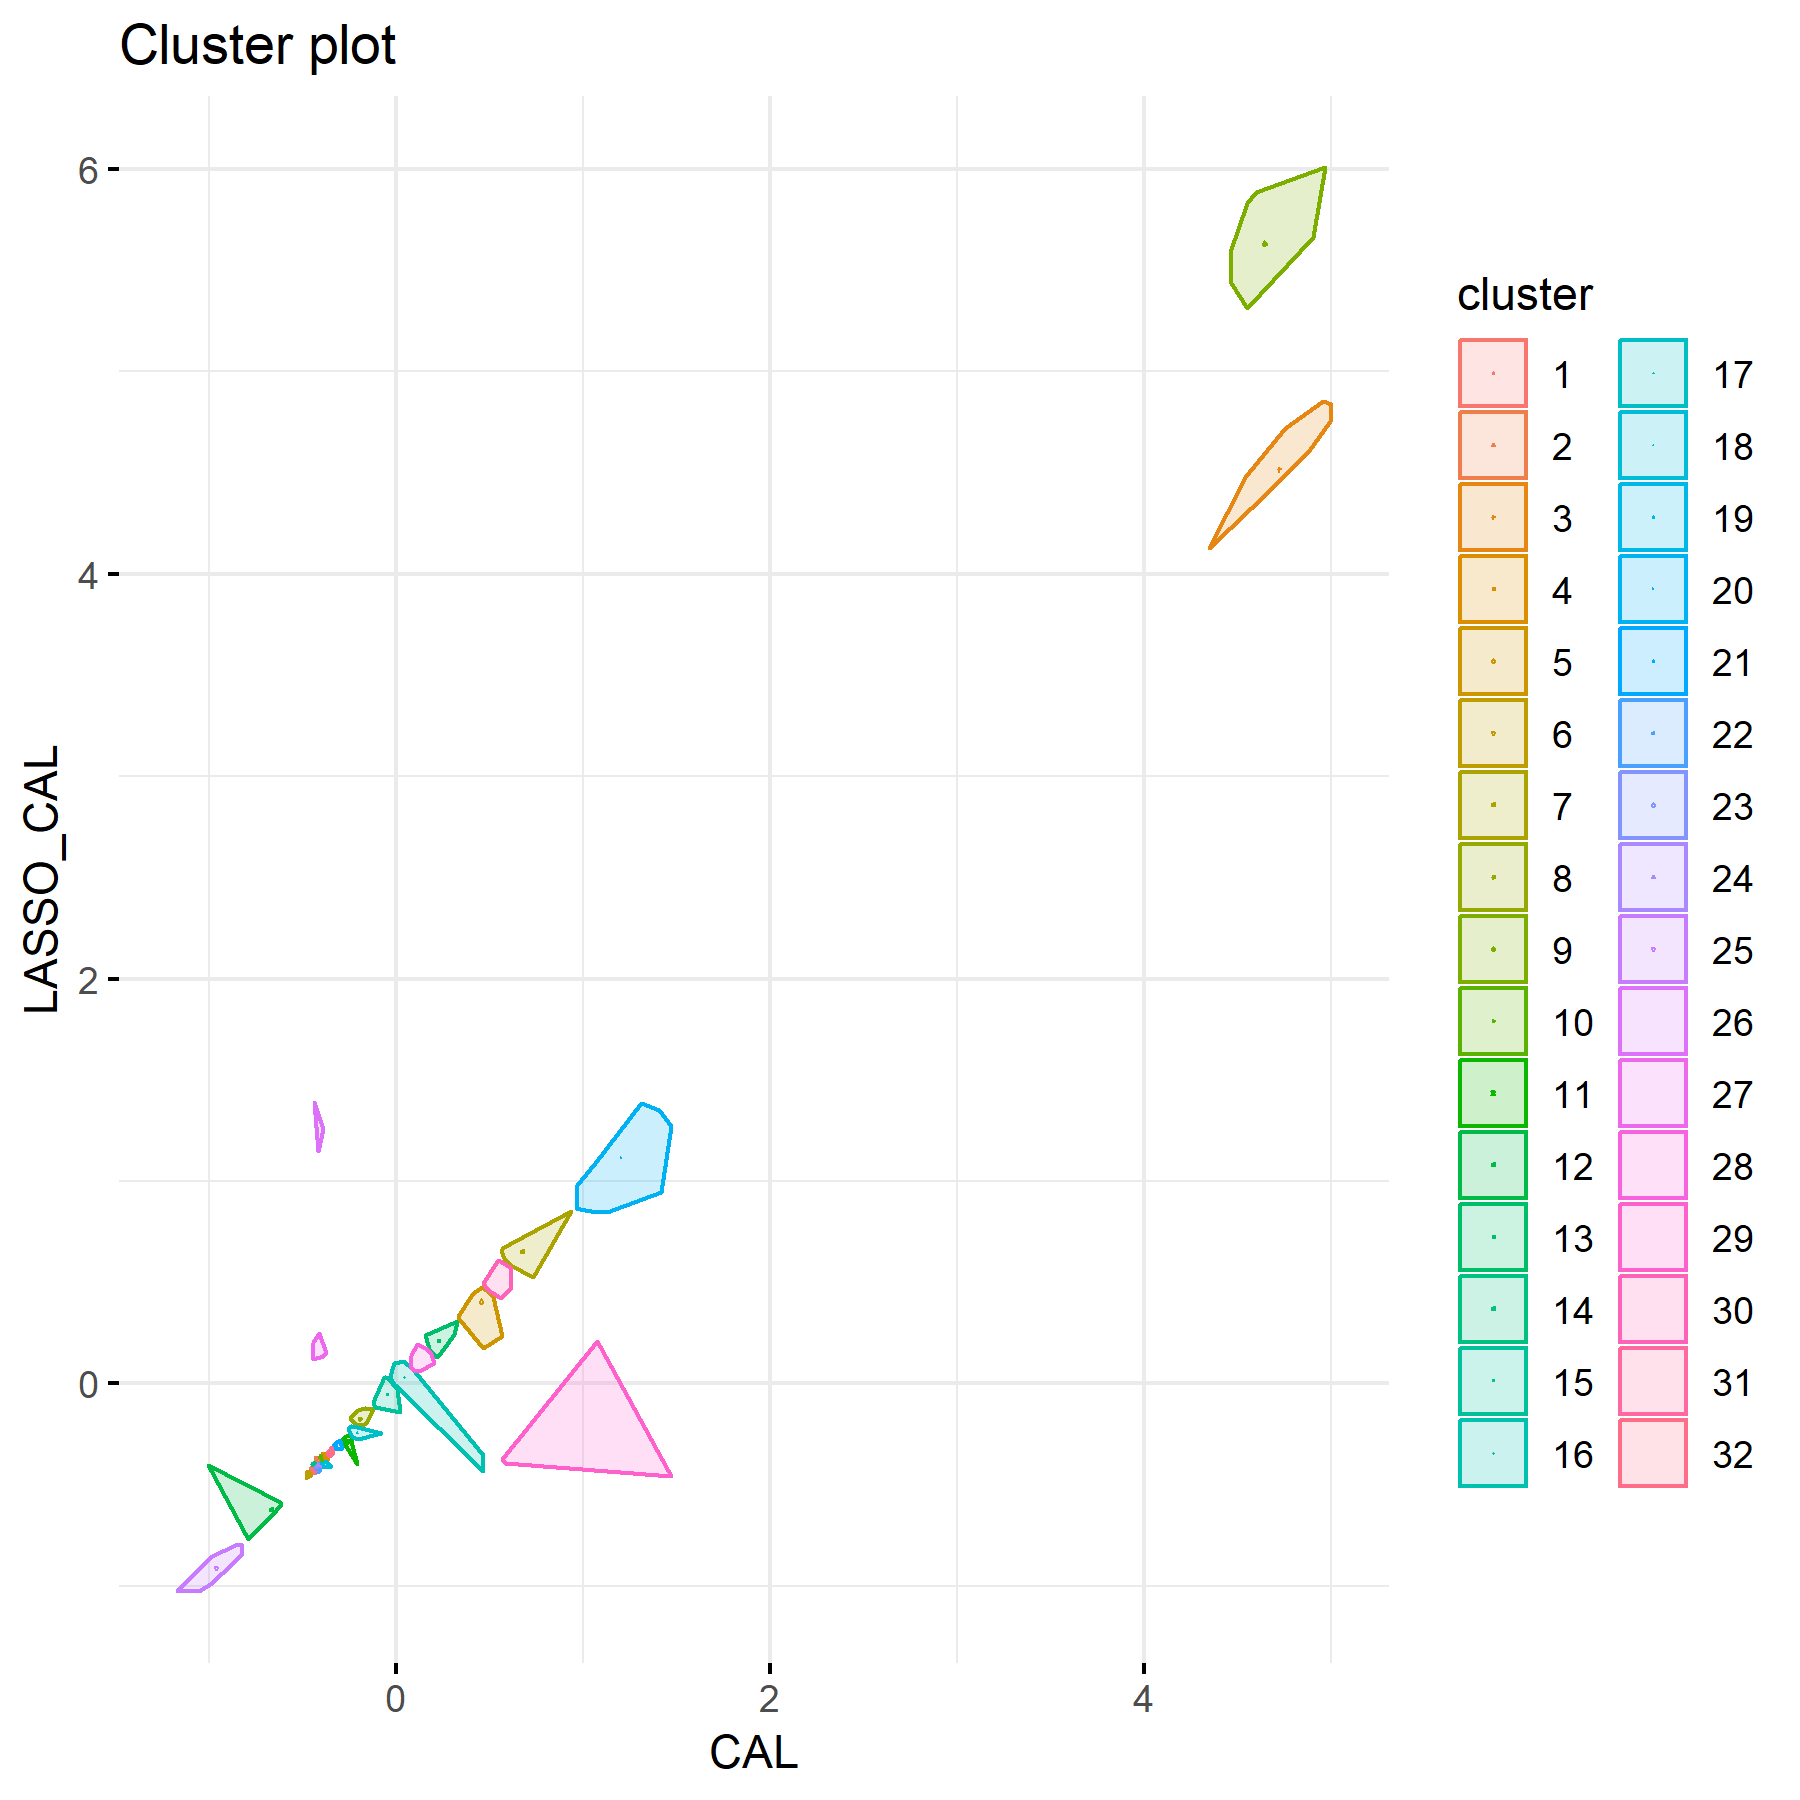
\includegraphics[width=0.48\textwidth]{../plot/cluster_CAL.png}
    \caption{K-means clustering result for all 3200 low track csv files, left side is for all estimation method, right side is for CAL and LASSO\_CAL}
    \label{fig:cluster1}
\end{figure}
Without specifying the cluster number, there were 27 clusters detected, 14 was identified for both LASSO\_CAL and LASSO\_AIPW methods, and both Random forest methods detect 8 clusters. However, these results serve no more than a possible measure of how well is the performance, especially without more knowledge of what the true ATEs are. 
\begin{figure}[h]
\centering
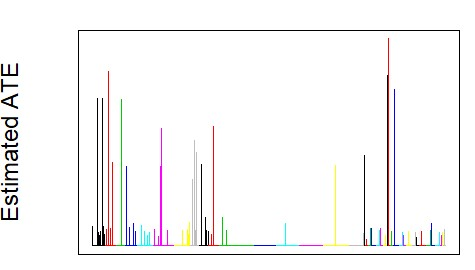
\includegraphics[width=0.65\textwidth]{../plot/cluster_uni.jpg}
    \caption{Univariate clustering result for LASSO\_CAL method only, detected 14 clusters.}
    \label{fig:cluster2}
\end{figure}

\section{Discussion}\label{sec:disc}
In this method we briefly compare seven methods, which can be characterized as either the basic model or the two-step. Based on the training set, calibration weights (CAL), as a non-parametric estimation process, outperforms other methods in most cases. In general, the two step methods performed better than the basic model. There are still a few questions left , including the actual algorithm performance on testing set, which is not accessible until the meeting ends. As for the methodology, other possible extensions including the usage of non-linear model for both outcome and propensity score, or add in the interaction terms into the modeling. Other variable selection methods, like elastic net(ENET), may also be applied. 

%
% ---- Bibliography ----
%
\newpage

\begin{thebibliography}{5}
\bibitem{Ashenfelter1978}
Ashenfelter, Orley. "Estimating the effect of training programs on earnings." The Review of Economics and Statistics (1978): 47-57.

\bibitem{Athey2019}
Athey, Susan, Julie Tibshirani, and Stefan Wager. "Generalized random forests." The Annals of Statistics 47.2 (2019): 1148-1178.

\bibitem{Chambers1992}
Chambers, John M., and Trevor J. Hastie, eds. Statistical models in S. Vol. 251. Pacific Grove, CA: Wadsworth \& Brooks/Cole Advanced Books \& Software, 1992.

\bibitem{Chan2016}
Chan, Kwun Chuen Gary, Sheung Chi Phillip Yam, and Zheng Zhang. "Globally efficient non‐parametric inference of average treatment effects by empirical balancing calibration weighting." Journal of the Royal Statistical Society: Series B (Statistical Methodology) 78.3 (2016): 673-700.

\bibitem{Chen2008}
Chen, Xiaohong, Han Hong, and Alessandro Tarozzi. "Semiparametric efficiency in GMM models with auxiliary data." The Annals of Statistics 36.2 (2008): 808-843.

\bibitem{Glynn2010}
Glynn, Adam N., and Kevin M. Quinn. "An introduction to the augmented inverse propensity weighted estimator." Political analysis 18.1 (2010): 36-56.

\bibitem{Imbens2004}
Imbens, Guido W. "Nonparametric estimation of average treatment effects under exogeneity: A review." Review of Economics and statistics 86.1 (2004): 4-29.

\bibitem{King2006}
King, Gary, and Langche Zeng. "The dangers of extreme counterfactuals." Political Analysis 14.2 (2006): 131-159.

\bibitem{LaLonde1986}
LaLonde, Robert J. "Evaluating the econometric evaluations of training programs with experimental data." The American economic review (1986): 604-620.

\bibitem{Luncefird2004}
Lunceford, Jared K., and Marie Davidian. "Stratification and weighting via the propensity score in estimation of causal treatment effects: a comparative study." Statistics in medicine 23.19 (2004): 2937-2960.

\bibitem{Oaxaca1973}
Oaxaca, Ronald. "Male-female wage differentials in urban labor markets." International economic review (1973): 693-709.

\bibitem{Pearl2002}
Pearl, Judea. "Causality: models, reasoning, and inference." IIE Transactions 34.6 (2002): 583-589.

\bibitem{Robins2000}
Robins, James M., Miguel Angel Hernan, and Babette Brumback. "Marginal structural models and causal inference in epidemiology." (2000): 550-560.

\bibitem{Rosenbaum1983}
Rosenbaum, Paul R., and Donald B. Rubin. "The central role of the propensity score in observational studies for causal effects." Biometrika 70.1 (1983): 41-55.
 
\bibitem{Rosenbaum1984}
Rosenbaum, Paul R., and Donald B. Rubin. "Reducing bias in observational studies using subclassification on the propensity score." Journal of the American statistical Association 79.387 (1984): 516-524.

\end{thebibliography}
\end{document}
